\chapter{\textit{The Fourth Dimension of Pythagoras: How Quadruples Crack Numbers}}
\label{ch12}



\bigskip


\begin{quote}
\itshape \textit{"Three dimensions are merely an invitation. Four is where the magic starts."}
\end{quote}


\bigskip


\section{A Puzzle in Four Parts}

I place four wooden blocks on the table in front of you. They are labelled $1$, $2$, $2$, and $3$. "Square each one," I say, "and add the first three." You oblige: $1^2 + 2^2 + 2^2 = 1 + 4 + 4 = 9 = 3^2$. Your eyebrows rise --- the sum of the first three squares is itself a perfect square, and it happens to equal the square of the fourth block.

"Cute," you say. "A coincidence."

I push four new blocks across the table: $2$, $3$, $6$, $7$. You check: $4 + 9 + 36 = 49 = 7^2$. Your eyebrows rise a little higher.

Now a challenge. I hand you a slip of paper that reads: *Find a quartet of positive integers $(a, b, c, d)$ such that $a^2 + b^2 + c^2 = d^2$ and $d = 9$.* I promise you that at least two solutions exist. Take a moment --- try pencil-and-paper before reading on. (Hints: one solution has $c = 8$; the other has $c = 7$.)

The answers are $(1, 4, 8, 9)$ and $(4, 4, 7, 9)$. Check them:

\[
1^2 + 4^2 + 8^2 = 1 + 16 + 64 = 81 = 9^2, \qquad 4^2 + 4^2 + 7^2 = 16 + 16 + 49 = 81 = 9^2.
\]

Both pass. And now we have a name for these creatures. A \textbf{Pythagorean quadruple} is any four-tuple $(a, b, c, d)$ of integers satisfying
\index{Pythagorean quadruple}

\[
a^2 + b^2 + c^2 = d^2.
\]

If the classical Pythagorean triple $a^2 + b^2 = c^2$ lives on a circle --- the set of all points at distance $c$ from the origin in a flat plane --- then a Pythagorean quadruple lives on a \textit{sphere}. The integer solutions to $a^2 + b^2 + c^2 = d^2$ are the lattice points on the surface of a ball of radius $d$ in three-dimensional space. But the equation itself, with its four variables, belongs naturally to the geometry of \textit{four} dimensions: the lattice points lie on the three-sphere $S^3$ inside $\mathbb{R}^4$.
\index{Pythagorean triple}
\index{lattice}

Here is a small gallery, sorted by hypotenuse, to whet the appetite:

\begin{center}
\begin{tabular}{c c c c c}
\toprule
$a$ & $b$ & $c$ & $d$ & Check \\
\midrule
$1$ & $2$ & $2$ & $3$ & $1+4+4=9$ \\
$2$ & $3$ & $6$ & $7$ & $4+9+36=49$ \\
$1$ & 4 & $8$ & $9$ & $1+16+64=81$ \\
$4$ & $4$ & $7$ & $9$ & $16+16+49=81$ \\
$1$ & $2$ & $14$ & $\!15\!$ & $1+4+196=201$? No! \\
\bottomrule
\end{tabular}
\end{center}

Wait --- that last row fails. $1 + 4 + 196 = 201 \neq 225$. The equation is pickier than it appears. Not every collection of four numbers will do. The constraint $a^2 + b^2 + c^2 = d^2$ is genuinely restrictive, and that selectivity is what makes quadruples \textit{useful}.

\begin{figure}[htbp]
\centering
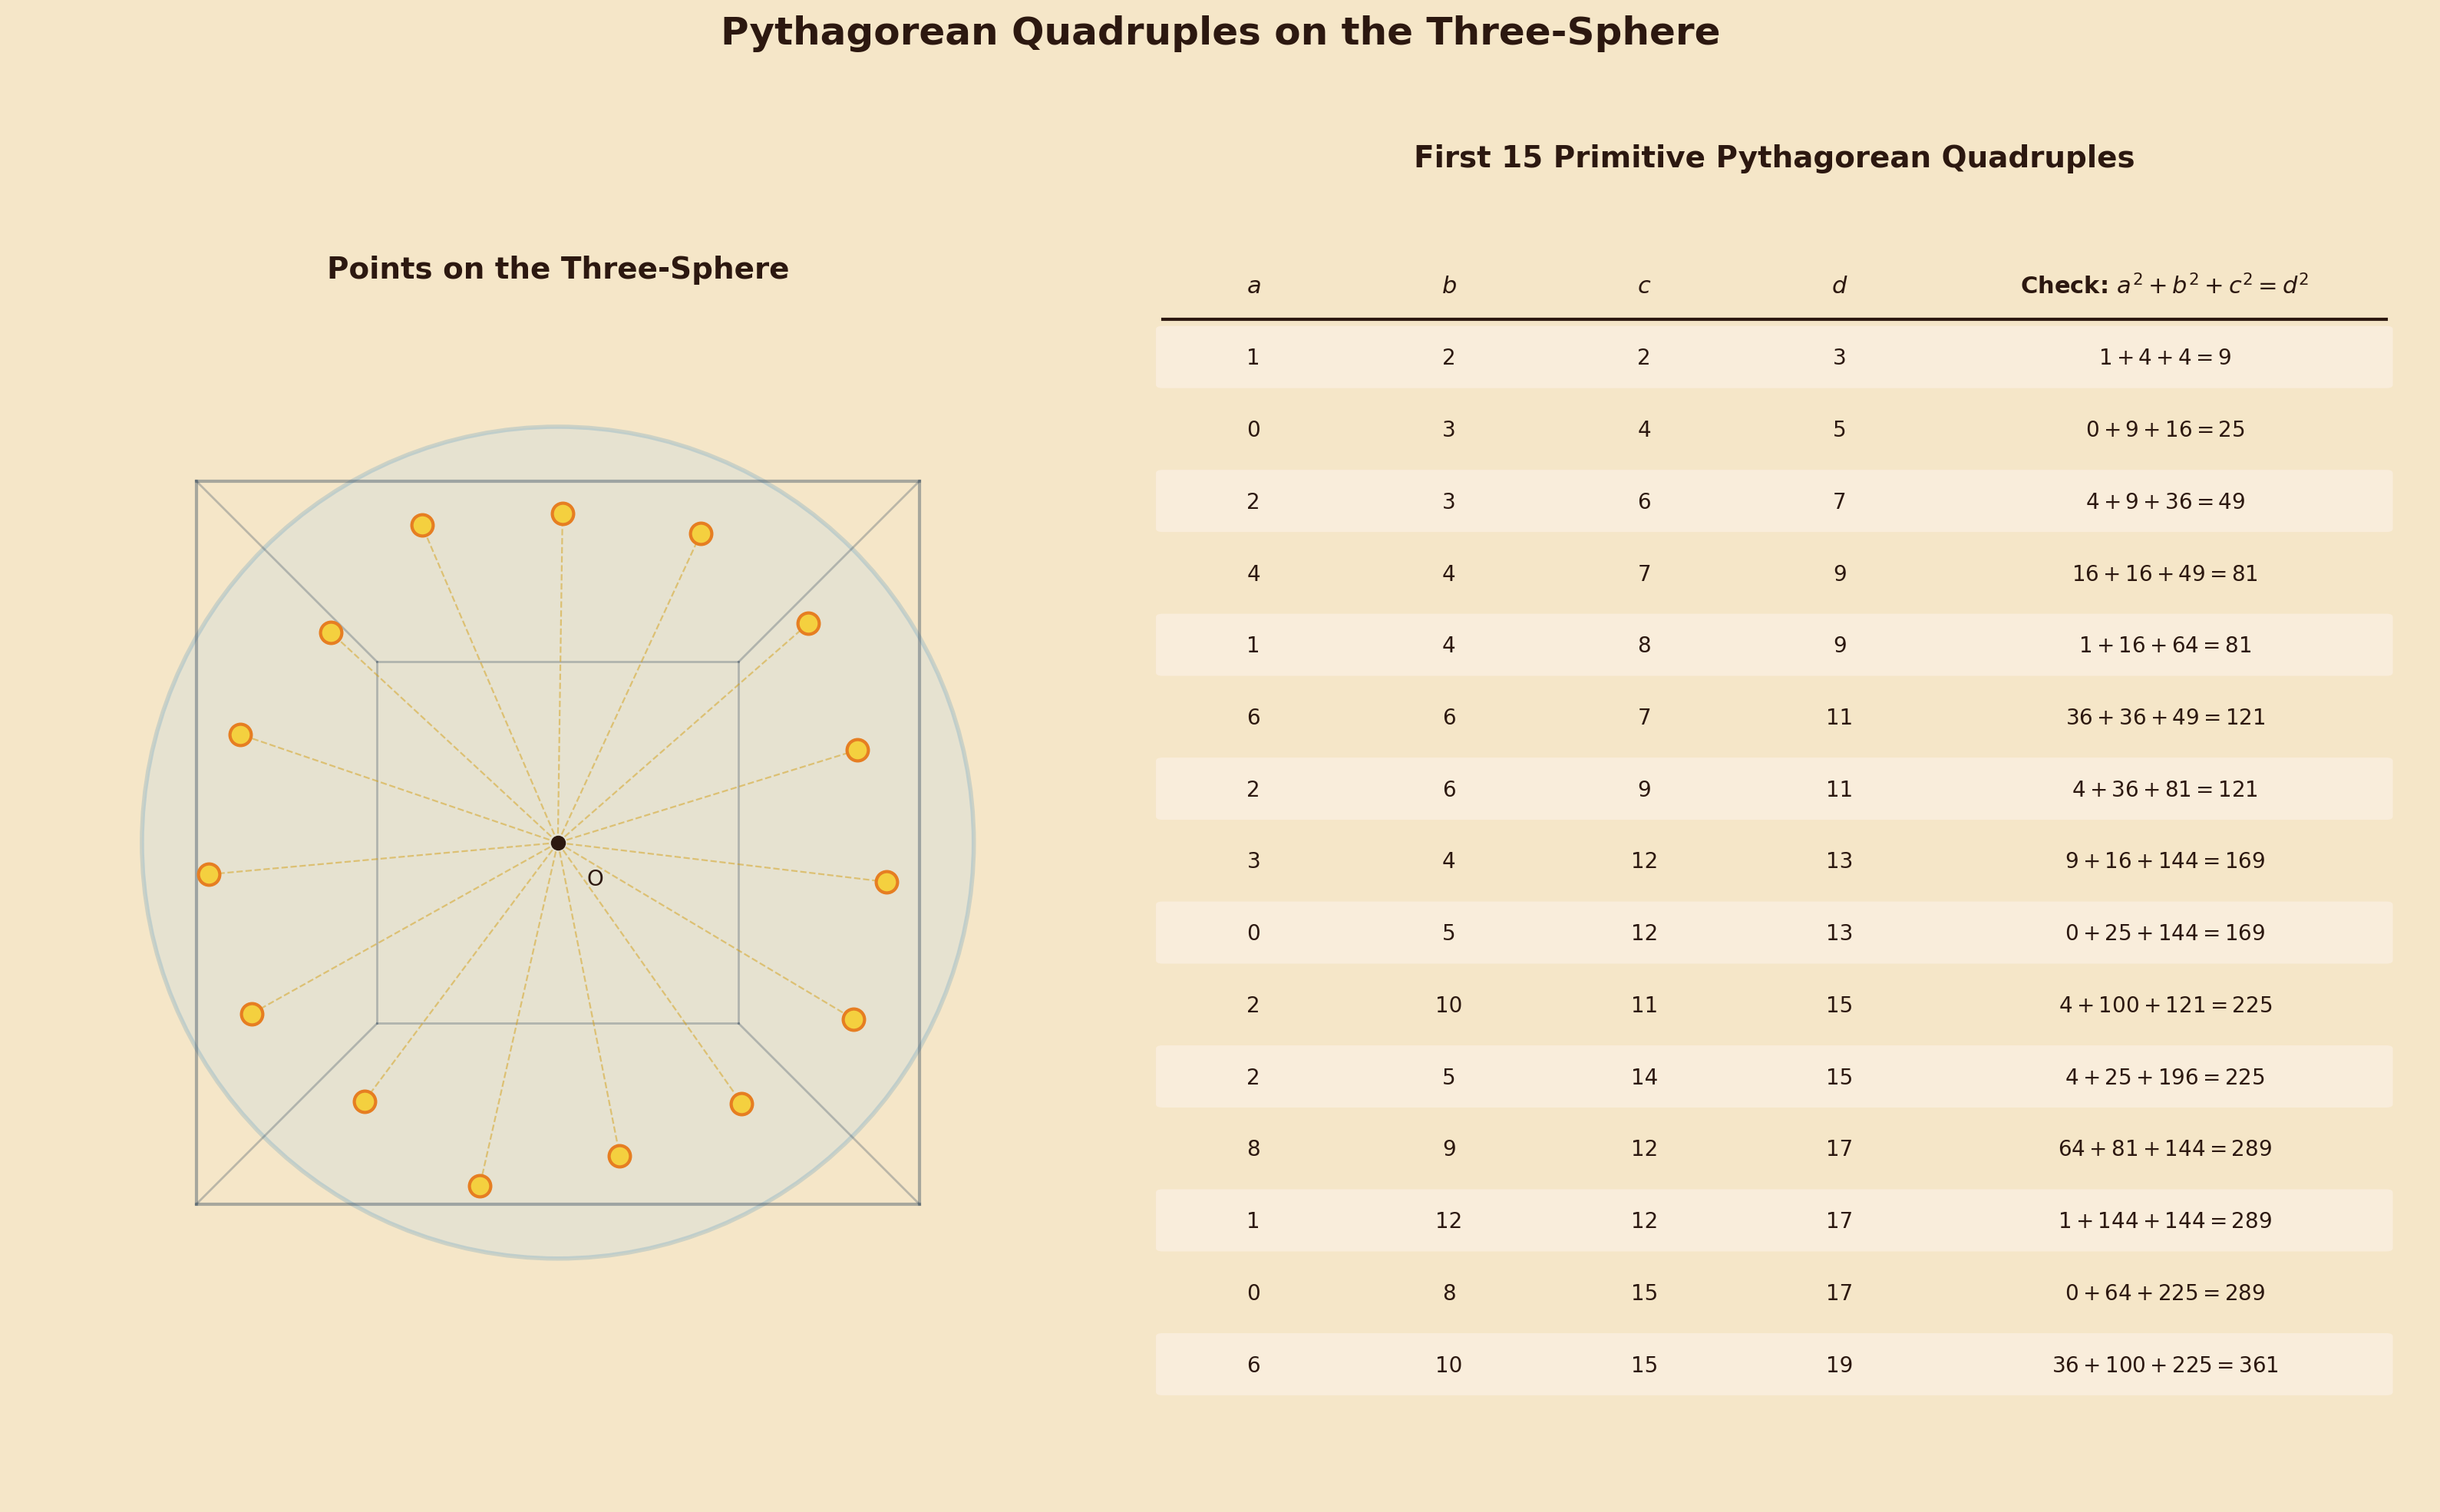
\includegraphics[width=0.82\textwidth]{../Chapter12/images/fig01_quadruple_table.png}
\caption{A beautifully arranged table of the first fifteen primitive Pythagorean quadruples (those with $\gcd(a,b,c,d)=1$), sorted by $d$, displayed inside a stylised four-dimensional hypercube wireframe.\ldots}
\end{figure}

\begin{figure}[htbp]
\centering
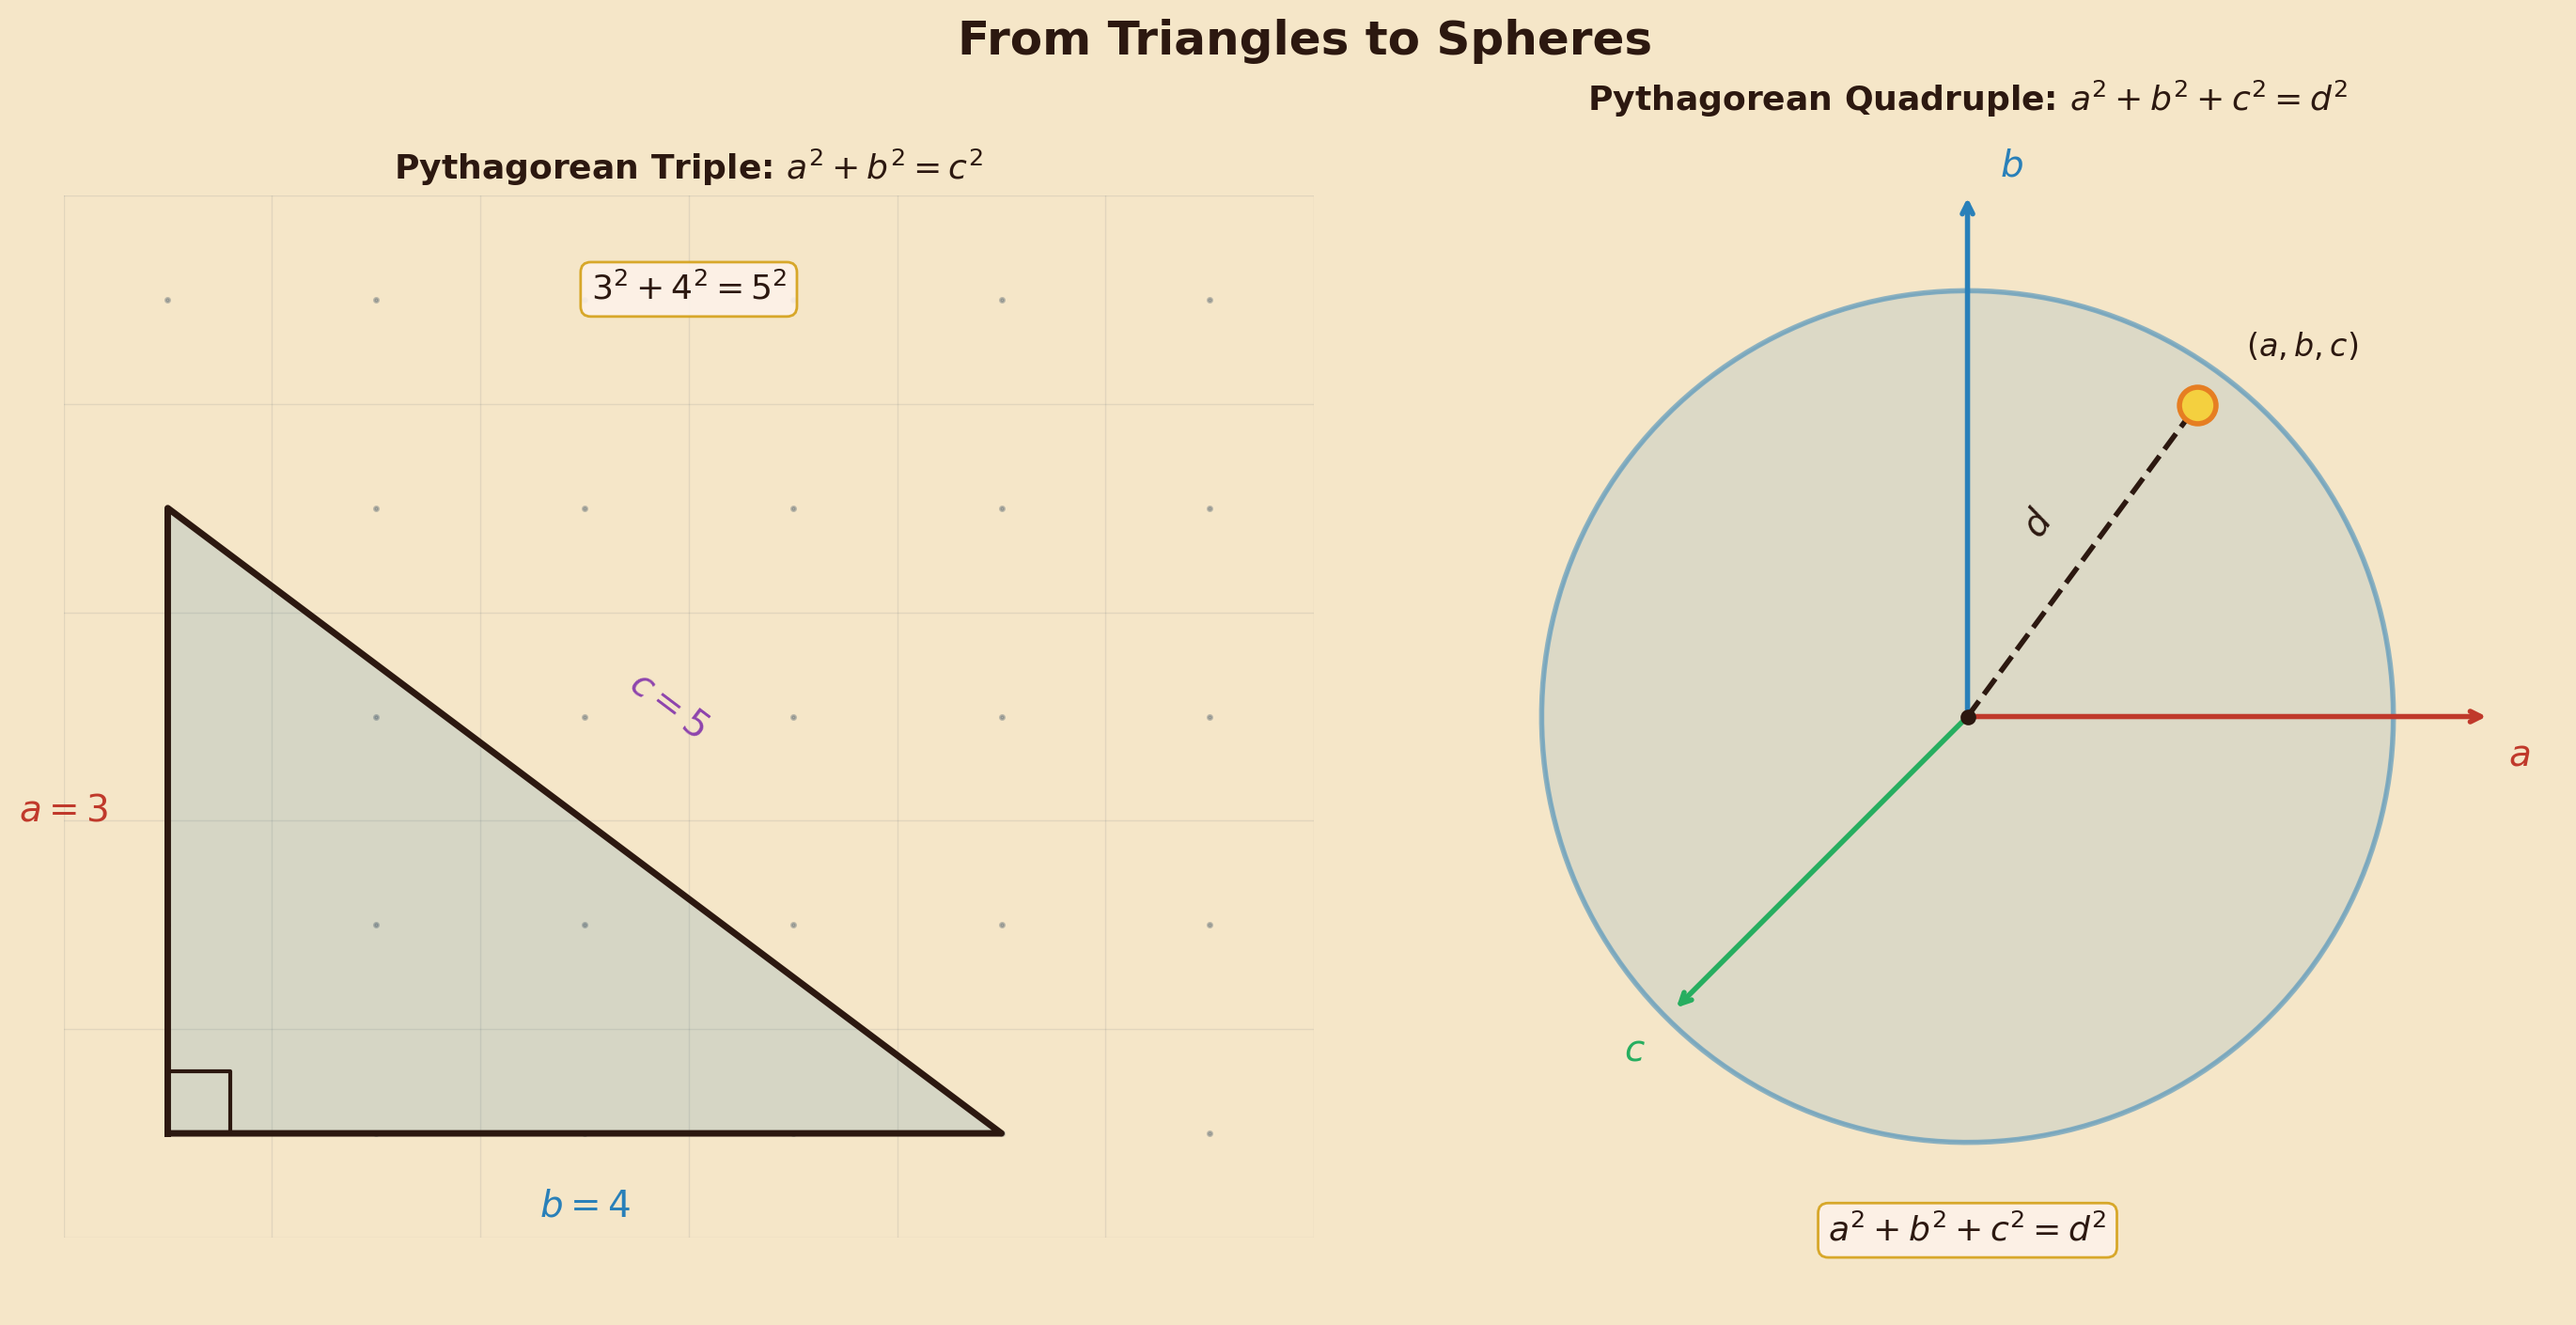
\includegraphics[width=0.82\textwidth]{../Chapter12/images/fig02_triangle_to_sphere.png}
\caption{Side-by-side comparison. Left panel: a right triangle inscribed on a flat integer grid, legs $a$ and $b$, hypotenuse $c$, illustrating $a^2 + b^2 = c^2$. Right panel: a tetrahedron-like projection\ldots}
\end{figure}

Euler studied sums of three squares; Jacobi counted the number of representations with exquisite generating-function machinery; Lagrange proved that every positive integer is a sum of four squares. The Pythagorean quadruple sits at the crossroads of these classical investigations. But it also harbours a secret that none of the old masters fully exploited: it is a \textit{factoring tool}. And that is what the rest of this chapter is about.
\index{factoring}
\index{Euler, Leonhard}


\bigskip


\section{The Magician's Bridge}

"I can factor $13$," I announce, "using nothing but the Pythagorean theorem in four dimensions."

You are understandably sceptical. Here is the trick. Start with the quadruple $(2, 3, 6, 7)$ and perform a single algebraic rearrangement:

\[
a^2 + b^2 = d^2 - c^2 = (d - c)(d + c).
\]

Substitute: $2^2 + 3^2 = (7 - 6)(7 + 6) = 1 \times 13 = 13$. The left side is a sum of two squares; the right side is a product of two factors. The bridge between \textit{geometry} (the Pythagorean equation) and \textit{arithmetic} (factoring) is a single equals sign.

Let us state this properly:

\begin{quote}
\itshape \textbf{The Difference-of-Squares Bridge.} For any Pythagorean quadruple $(a, b, c, d)$: $$(d - c)(d + c) = a^2 + b^2.$$
\end{quote}

The proof is one line: $d^2 - c^2 = (d^2 - c^2)$, and by the quadruple equation, $d^2 - c^2 = a^2 + b^2$. Factor the left side. Done.

Why should you care? Because every modern factoring algorithm --- the Quadratic Sieve, the Number Field Sieve, the methods that keep cryptographers awake at night --- boils down, at its mathematical core, to finding a \textit{difference of two squares} modulo a target number. A Pythagorean quadruple hands you one for free.

But the gift has varying generosity. Consider our two quadruples with $d = 9$:

\begin{itemize}
\item From $(1, 4, 8, 9)$: $(9 - 8)(9 + 8) = 1 \times 17 = 17$. The factor $d - c = 1$ is trivial --- we learn nothing.
\item From $(4, 4, 7, 9)$: $(9 - 7)(9 + 7) = 2 \times 16 = 32$. Now both factors exceed $1$. We have a \textit{non-trivial} factorisation of $32 = 4^2 + 4^2$.
\end{itemize}
Same hypotenuse, wildly different factoring behaviour! The first quadruple's "legs" are too unbalanced --- $c$ is so close to $d$ that the gap $d - c$ collapses to $1$. The second quadruple distributes its energy more evenly, and the payoff is richer. This observation --- that \textit{balanced} quadruples are better factoring tools --- will become a recurring theme.

\begin{figure}[htbp]
\centering
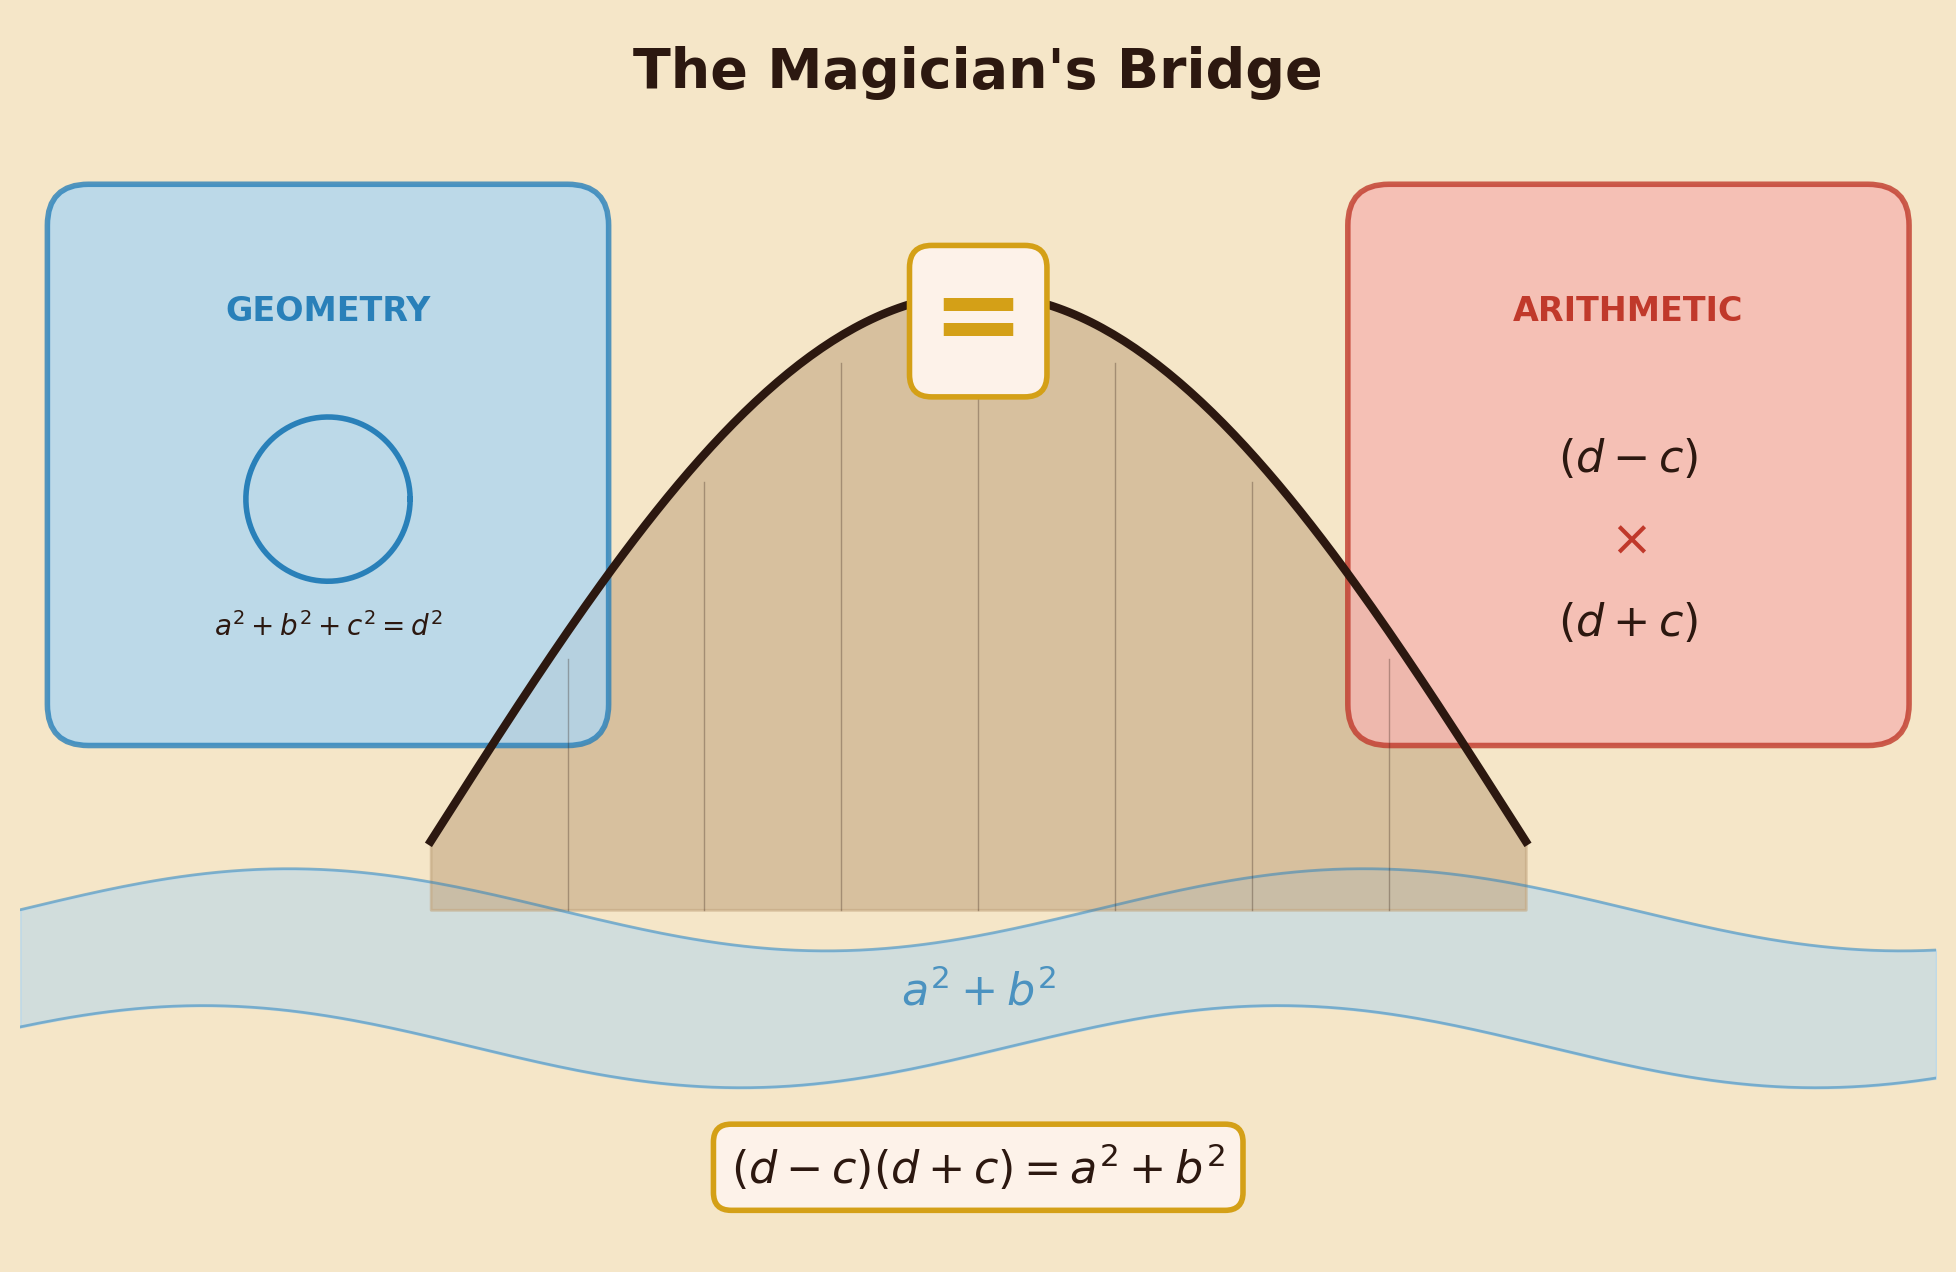
\includegraphics[width=0.82\textwidth]{../Chapter12/images/fig03_bridge.png}
\caption{A stone arch bridge spanning a river. On the left bank stands a translucent sphere labelled "$a^2 + b^2 + c^2 = d^2$" with the word "GEOMETRY" beneath. On the right bank, two parenthetical\ldots}
\end{figure}


\bigskip


\section{The Master Key}

"I'll give you four knobs," I say, gesturing at an imaginary machine. "Label them $m$, $n$, $p$, $q$. Turn each knob to any integer setting you like, and I will hand you a valid Pythagorean quadruple --- guaranteed, no exceptions, no fine print."

Try it: set $m = 1$, $n = 1$, $p = 1$, $q = 0$. The machine whirs and produces:

\[
\begin{aligned}
a &= m^2 + n^2 - p^2 - q^2 = 1 + 1 - 1 - 0 = 1, \\
b &= 2(mq + np) = 2(0 + 1) = 2, \\
c &= 2(nq - mp) = 2(0 - 1) = -2, \\
d &= m^2 + n^2 + p^2 + q^2 = 1 + 1 + 1 + 0 = 3.
\end{aligned}
\]

Check: $1^2 + 2^2 + (-2)^2 = 1 + 4 + 4 = 9 = 3^2$. Our old friend $(1, 2, 2, 3)$, with a sign flip on $c$ (which does not affect the equation, since $c$ appears squared). The machine works.

Here is the parametric representation in full:

\[
\boxed{\begin{aligned}
a &= m^2 + n^2 - p^2 - q^2, \\
b &= 2(mq + np), \\
c &= 2(nq - mp), \\
d &= m^2 + n^2 + p^2 + q^2.
\end{aligned}}
\]

Why does this always produce a valid quadruple? The verification is pure bookkeeping --- expand $a^2 + b^2 + c^2$ and $d^2$ separately, and watch the cross-terms cancel. The reader armed with patience and a large sheet of paper can confirm every step. The key miracle is that $d^2 = (m^2 + n^2 + p^2 + q^2)^2$ expands into exactly the same sixteen terms as $a^2 + b^2 + c^2$.

But the \textit{real} revelation is what the machine tells us about the hypotenuse:

\[
d = (m^2 + n^2) + (p^2 + q^2).
\]

The hypotenuse decomposes as a sum of two "norms" --- two sums-of-two-squares. This is precisely the structure Euler exploited in the 18th century to factor large numbers. The four parameters $(m, n, p, q)$ look suspiciously like the components of a \textit{quaternion}, and indeed the connection is deep and genuine. Hamilton's four-dimensional number system is not a historical curiosity; it is the algebraic engine behind the parametric machine.
\index{quaternions}
\index{Hamilton, William Rowan}

\begin{figure}[htbp]
\centering
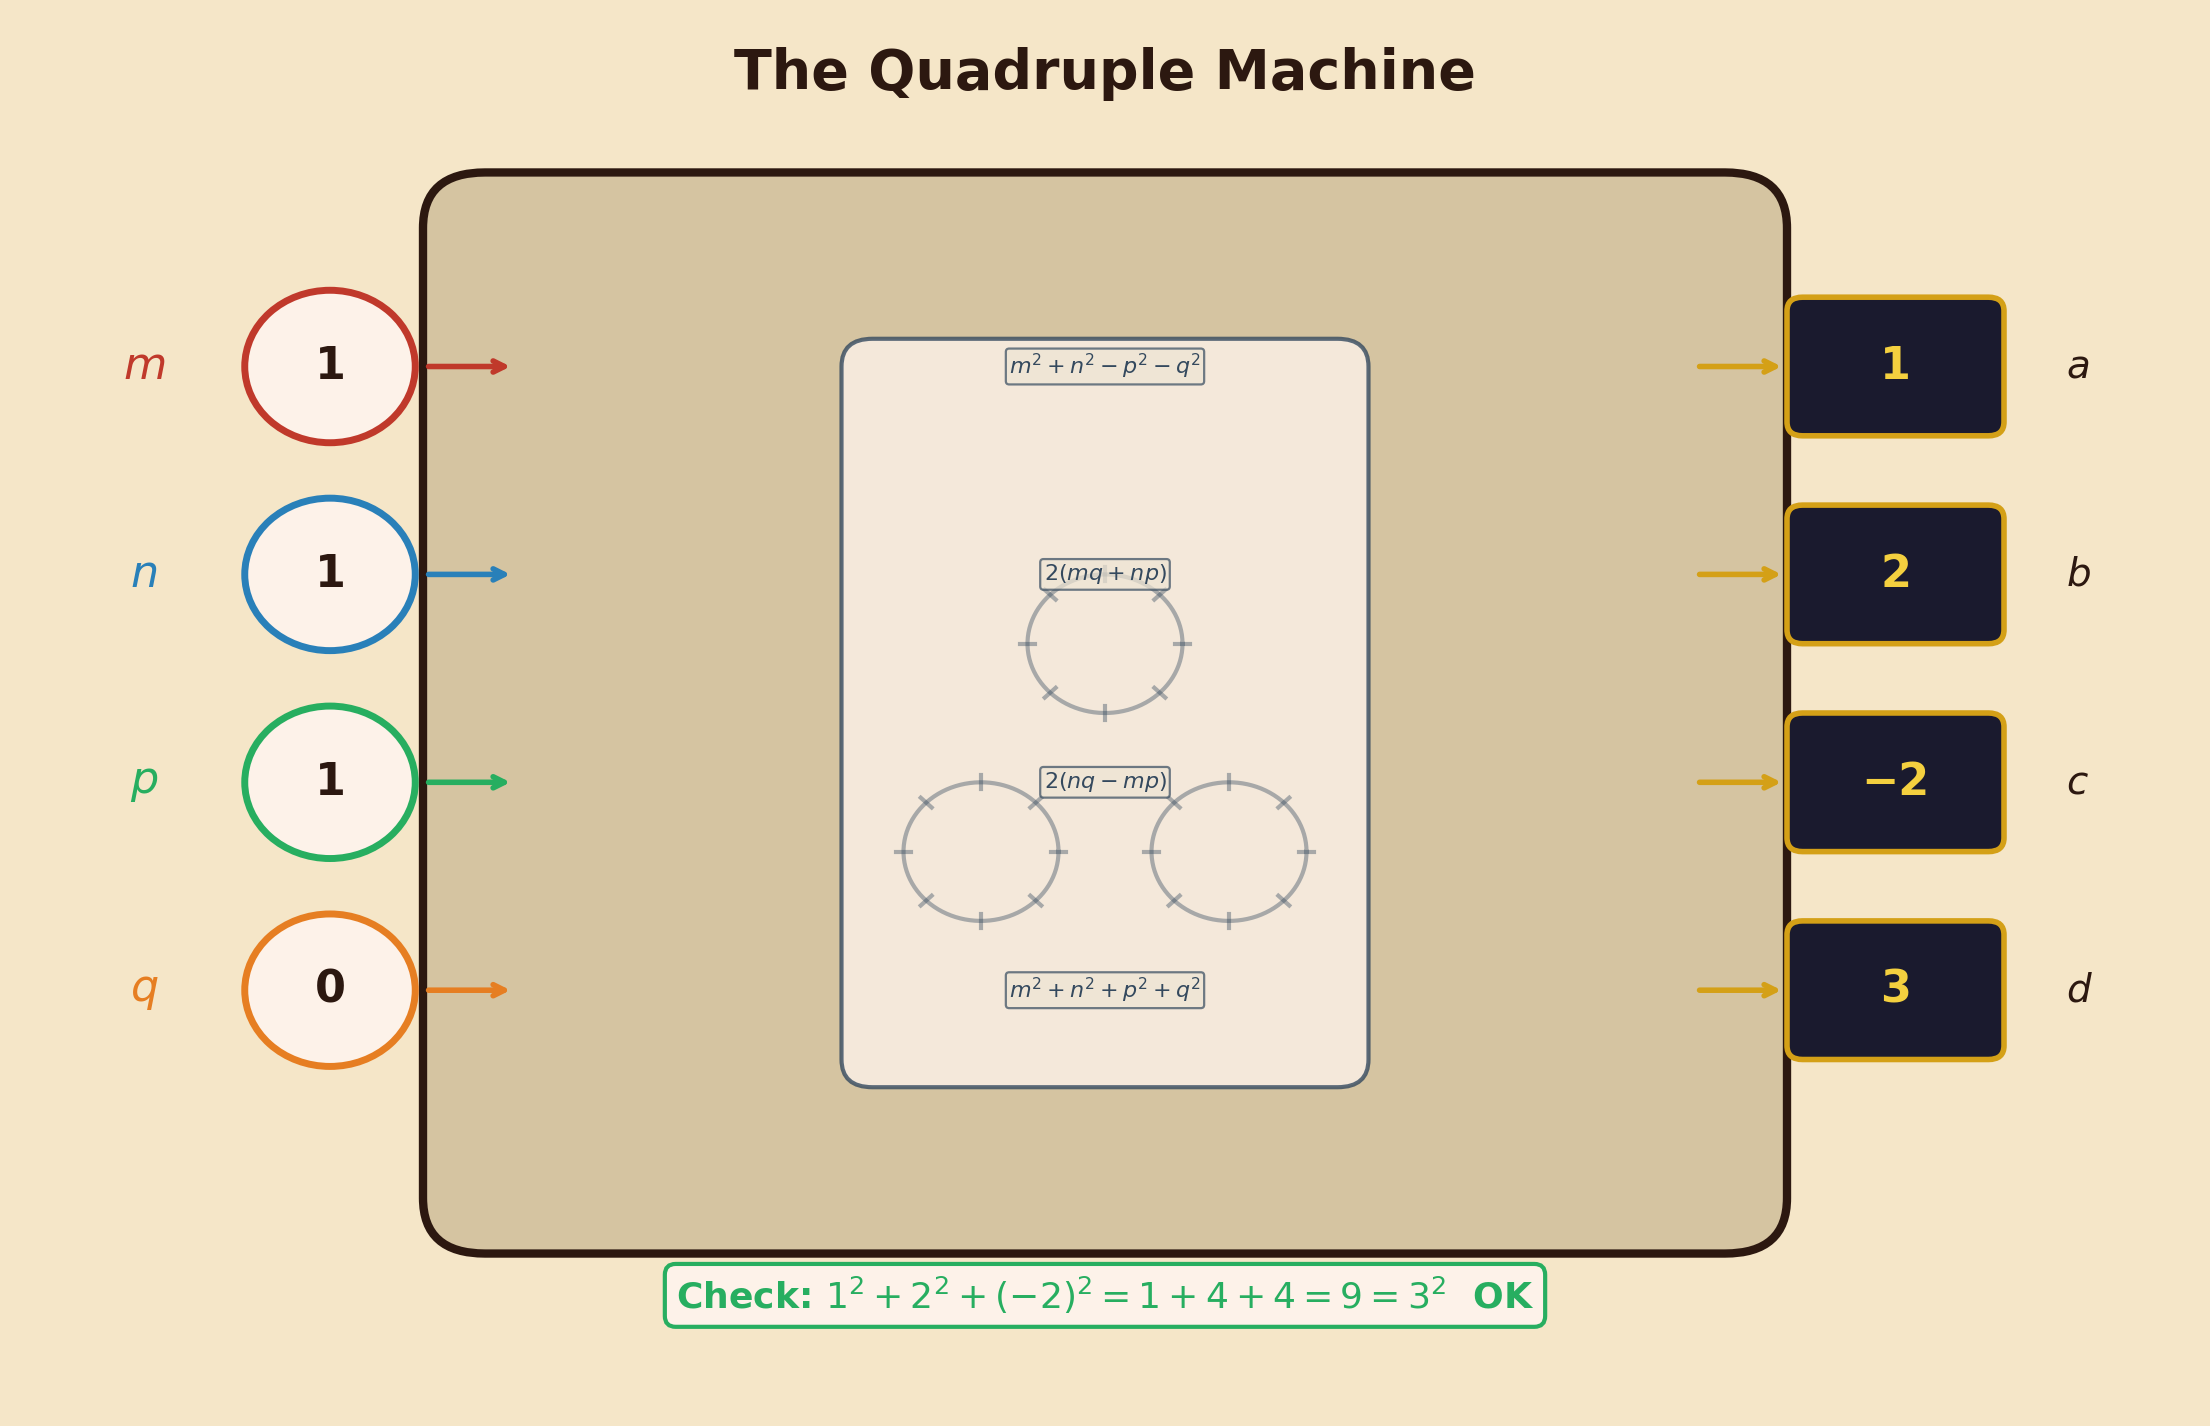
\includegraphics[width=0.82\textwidth]{../Chapter12/images/fig04_quadruple_machine.png}
\caption{A vintage brass-and-mahogany mechanical device with four labelled input dials ($m$, $n$, $p$, $q$) on the left and four output displays ($a$, $b$, $c$, $d$) on the right. Interlocking gears connect\ldots}
\end{figure}

\begin{figure}[htbp]
\centering
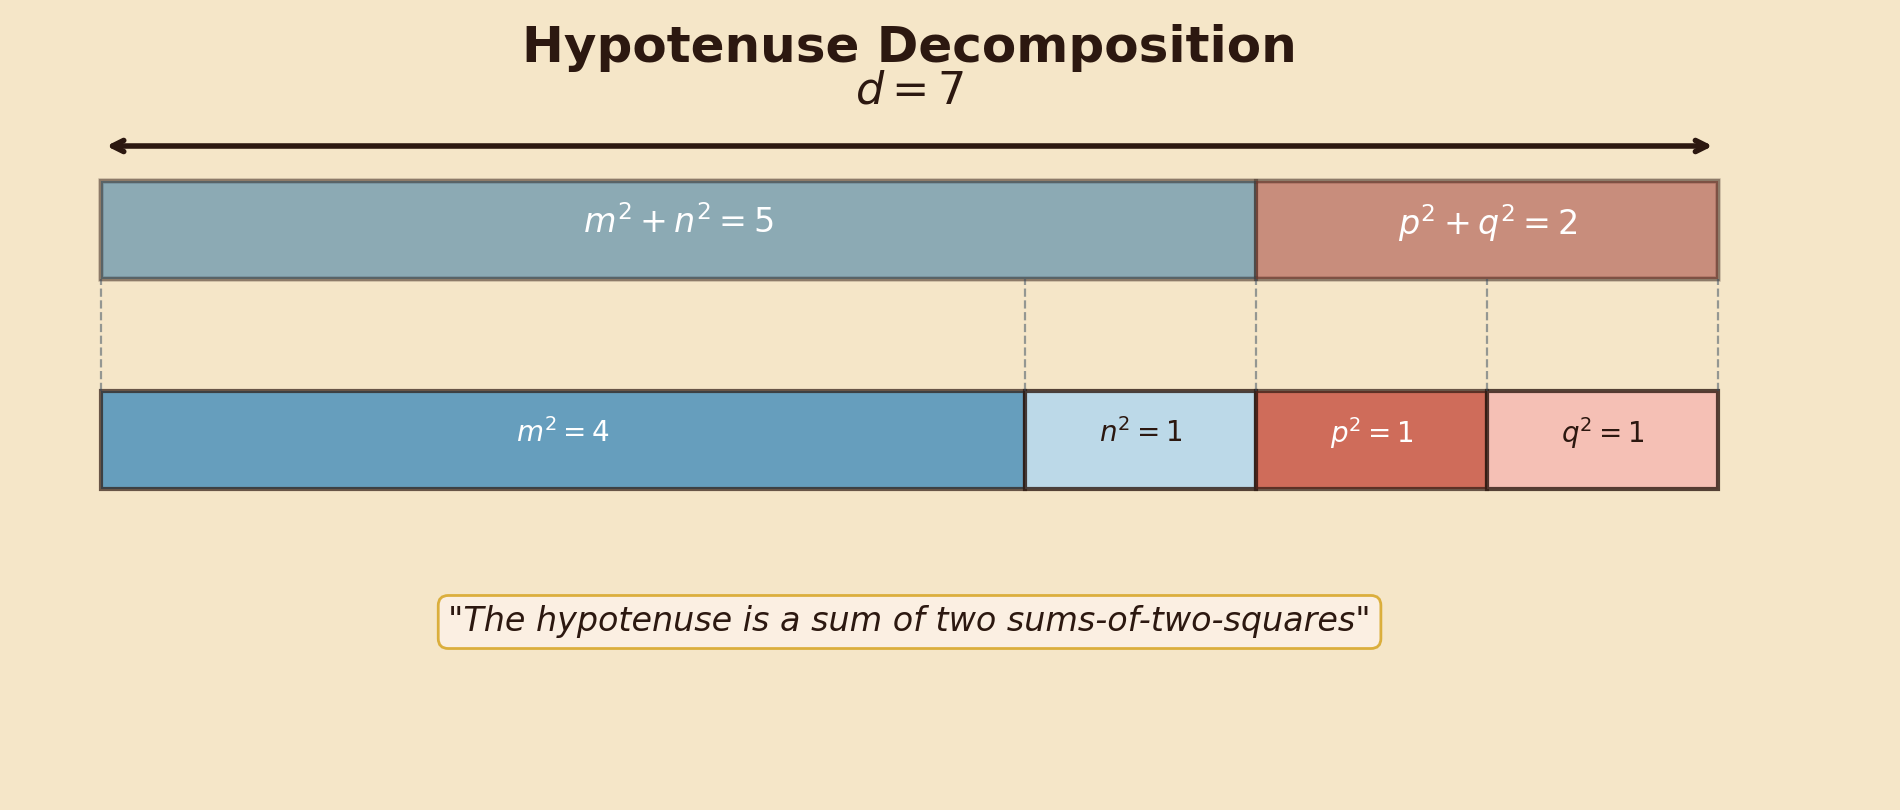
\includegraphics[width=0.82\textwidth]{../Chapter12/images/fig05_hypotenuse_decomposition.png}
\caption{A number-line diagram showing $d$ as a single segment, decomposed into two coloured sub-segments: $m^2 + n^2$ (shaded blue) and $p^2 + q^2$ (shaded red). Each sub-segment is further subdivided into\ldots}
\end{figure}


\bigskip


\section{The Collision Detector}

$81$ can be written as a sum of three squares in at least two ways:

\[
81 = 1^2 + 4^2 + 8^2 = 4^2 + 4^2 + 7^2.
\]

Is this an accident --- or a weapon?

It is a weapon. When two different Pythagorean quadruples share the same hypotenuse $d$, their coexistence creates a \textit{collision} --- and collisions leak factoring information. Here is the mechanism.

Suppose $(a_1, b_1, c_1, d)$ and $(a_2, b_2, c_2, d)$ are two quadruples with the same hypotenuse. Then:

\[
a_1^2 + b_1^2 + c_1^2 = d^2 = a_2^2 + b_2^2 + c_2^2.
\]

Subtract: $c_1^2 - c_2^2 = (a_2^2 - a_1^2) + (b_2^2 - b_1^2)$. Factor the left side:

\[
(c_1 - c_2)(c_1 + c_2) = (a_2^2 - a_1^2) + (b_2^2 - b_1^2).
\]

For our pair with $d = 9$: $(8 - 7)(8 + 7) = 1 \times 15 = 15$. And $(16 - 1) + (16 - 16) = 15$. Check. Now compute $\gcd(15, 81) = 3$ --- and we have extracted a factor of $81 = 3^4$.

The word "collision" is deliberate: this is the same principle behind \textit{birthday attacks} in cryptography. Finding two representations of the same number as a sum of three squares is the number-theoretic analogue of finding a hash collision --- and just as devastating.

\begin{figure}[htbp]
\centering
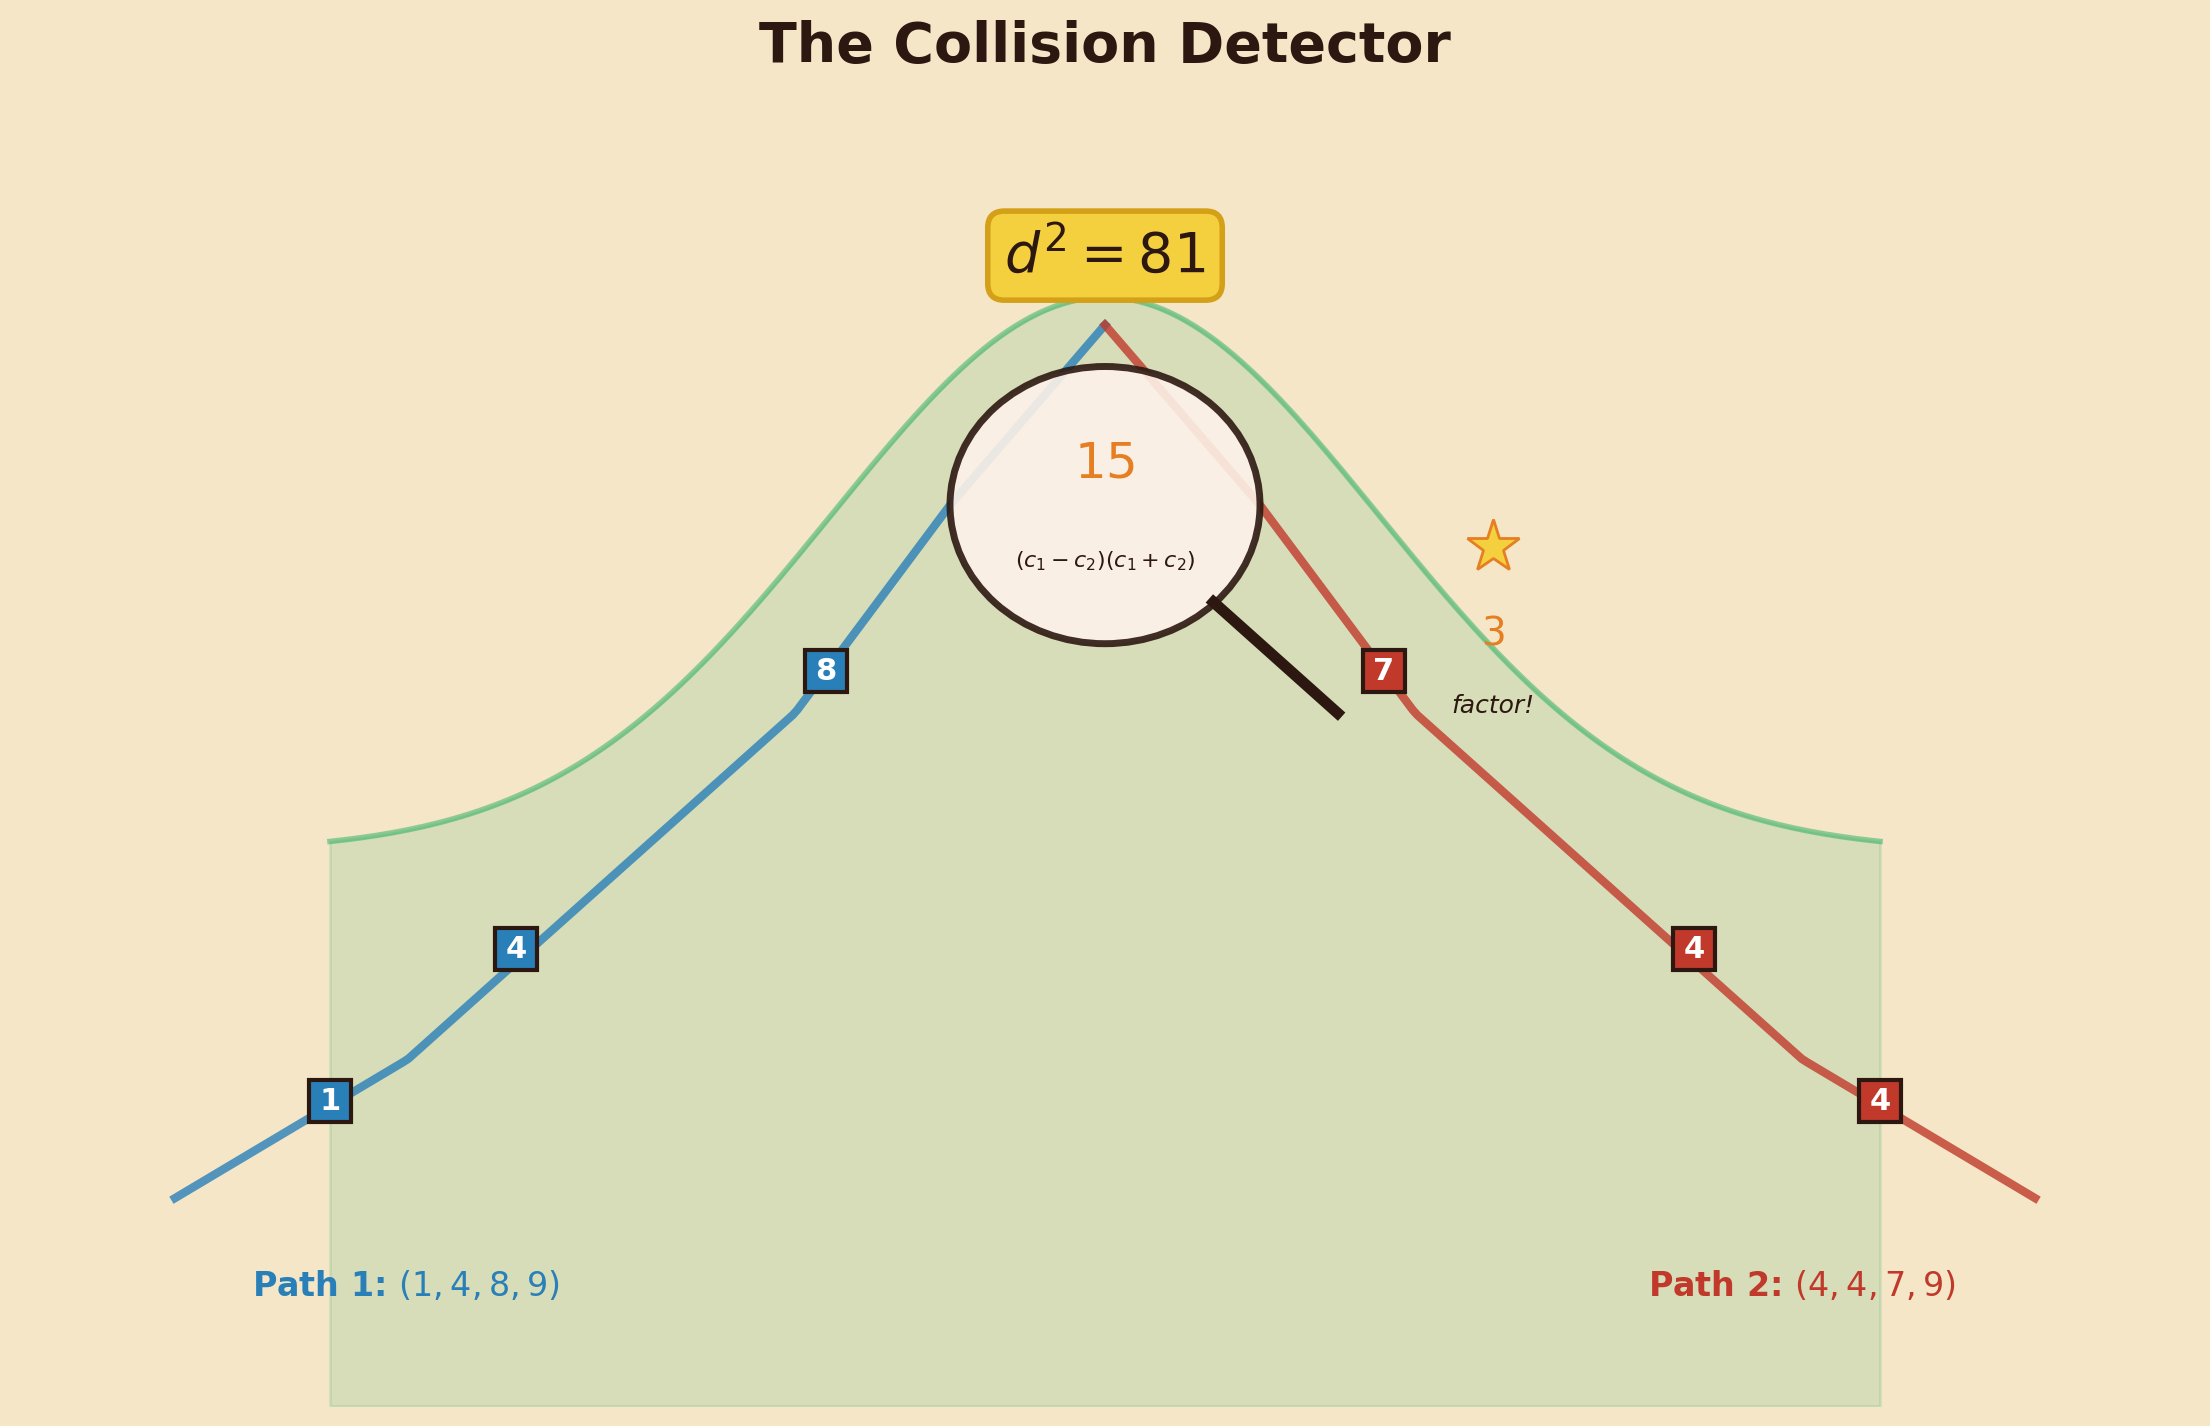
\includegraphics[width=0.82\textwidth]{../Chapter12/images/fig06_collision_roads.png}
\caption{Two winding roads on a hilly landscape, each starting from a different village, converge on the same hilltop labelled $d^2 = 81$. The left road is marked with milestones $1$, $4$, $8$ (the components\ldots}
\end{figure}


\bigskip


\section{Stretching the Quadruple}

If $(1, 2, 2, 3)$ is a Pythagorean quadruple, then so is $(10, 20, 20, 30)$ --- just multiply every component by $10$. Obvious, perhaps. But this "trivial" observation is the seed of a powerful technique.

\begin{quote}
\itshape \textbf{The Scaling Lemma.} If $(a, b, c, d)$ satisfies $a^2 + b^2 + c^2 = d^2$, then for any integer $k$: $$(ka)^2 + (kb)^2 + (kc)^2 = (kd)^2.$$
\end{quote}

The proof is one line of algebra: $k^2 a^2 + k^2 b^2 + k^2 c^2 = k^2(a^2 + b^2 + c^2) = k^2 d^2 = (kd)^2$.

The converse operation is just as important: any common factor $g = \gcd(a, b, c, d)$ can be divided out, reducing the quadruple to a \textit{primitive} one --- a quadruple whose four components share no common factor greater than $1$. The study of all quadruples thus reduces to the study of primitive quadruples, just as in the theory of Pythagorean triples.

A subtle point: scaling the \textit{parameters} $(m, n, p, q)$ of the machine by $k$ does not scale the quadruple by $k$ --- it scales the quadruple by $k^2$. The parametric machine squares its inputs before combining them, so parameter-scaling and quadruple-scaling are related by a square. This asymmetry will matter when we attempt to reverse-engineer the parameters from a given quadruple.

\begin{figure}[htbp]
\centering
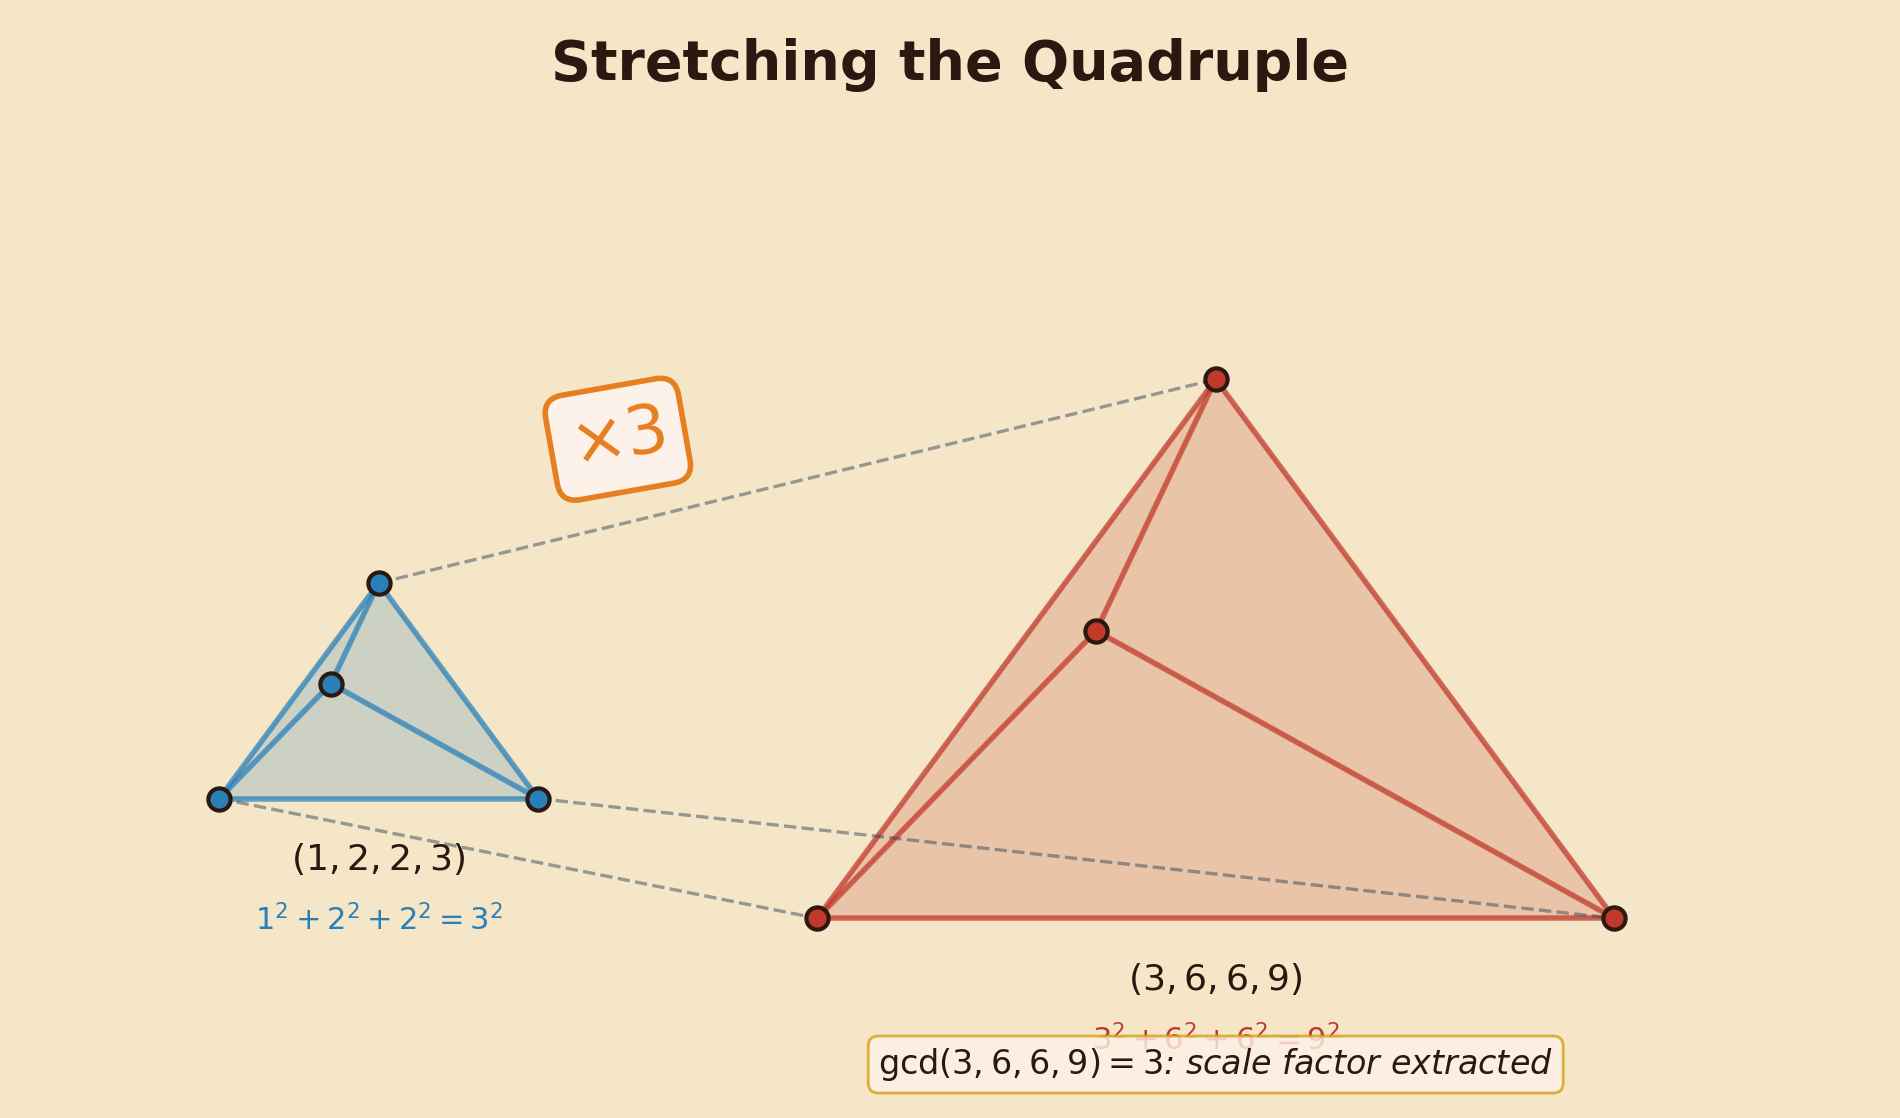
\includegraphics[width=0.82\textwidth]{../Chapter12/images/fig07_scaling_tetrahedra.png}
\caption{A small tetrahedron with vertices labelled $(1, 2, 2, 3)$ sits beside a geometrically similar but three-times-larger tetrahedron labelled $(3, 6, 6, 9)$. Dotted lines connect corresponding vertices.\ldots}
\end{figure}


\bigskip


\section{The Lattice Detective}

Two Pythagorean quadruples share the hypotenuse $d = 9$:

\[
(1, 4, 8, 9) \qquad \text{and} \qquad (4, 4, 7, 9).
\]

Here is a curious exercise. Compute $(1 - 4)(1 + 4) + (4 - 4)(4 + 4)$. You get $(-3)(5) + (0)(8) = -15$. Now compute $(7 - 8)(7 + 8) = (-1)(15) = -15$. The same number! Is this a coincidence?

It is not. For any two quadruples $(a_1, b_1, c_1, d)$ and $(a_2, b_2, c_2, d)$ sharing the same hypotenuse:

\[
(a_1 - a_2)(a_1 + a_2) + (b_1 - b_2)(b_1 + b_2) = (c_2 - c_1)(c_2 + c_1).
\]

This is the \textbf{Lattice Pair Identity} --- the "cross-examination" of two witnesses who both claim to have seen the number $d^2$. Their testimony must be \textit{consistent}, and the consistency condition encodes factoring information in the cross-differences.

The word "lattice" is chosen deliberately. The set of all integer points $(a, b, c)$ on the sphere $a^2 + b^2 + c^2 = d^2$ forms a finite subset of the integer lattice $\mathbb{Z}^3$. Pairs of such lattice points, connected by the identity above, trace out a web of algebraic relationships --- a detective's string-and-pushpin board, with every thread taut with arithmetic meaning.

A Gardner-style challenge: if three quadruples share the same hypotenuse, pairwise application of the Lattice Pair Identity yields $\binom{3}{2} = 3$ independent identities. Can more witnesses yield \textit{more} information? Always --- and the more representations $d^2$ possesses, the tighter the net draws around its factors.

\begin{figure}[htbp]
\centering
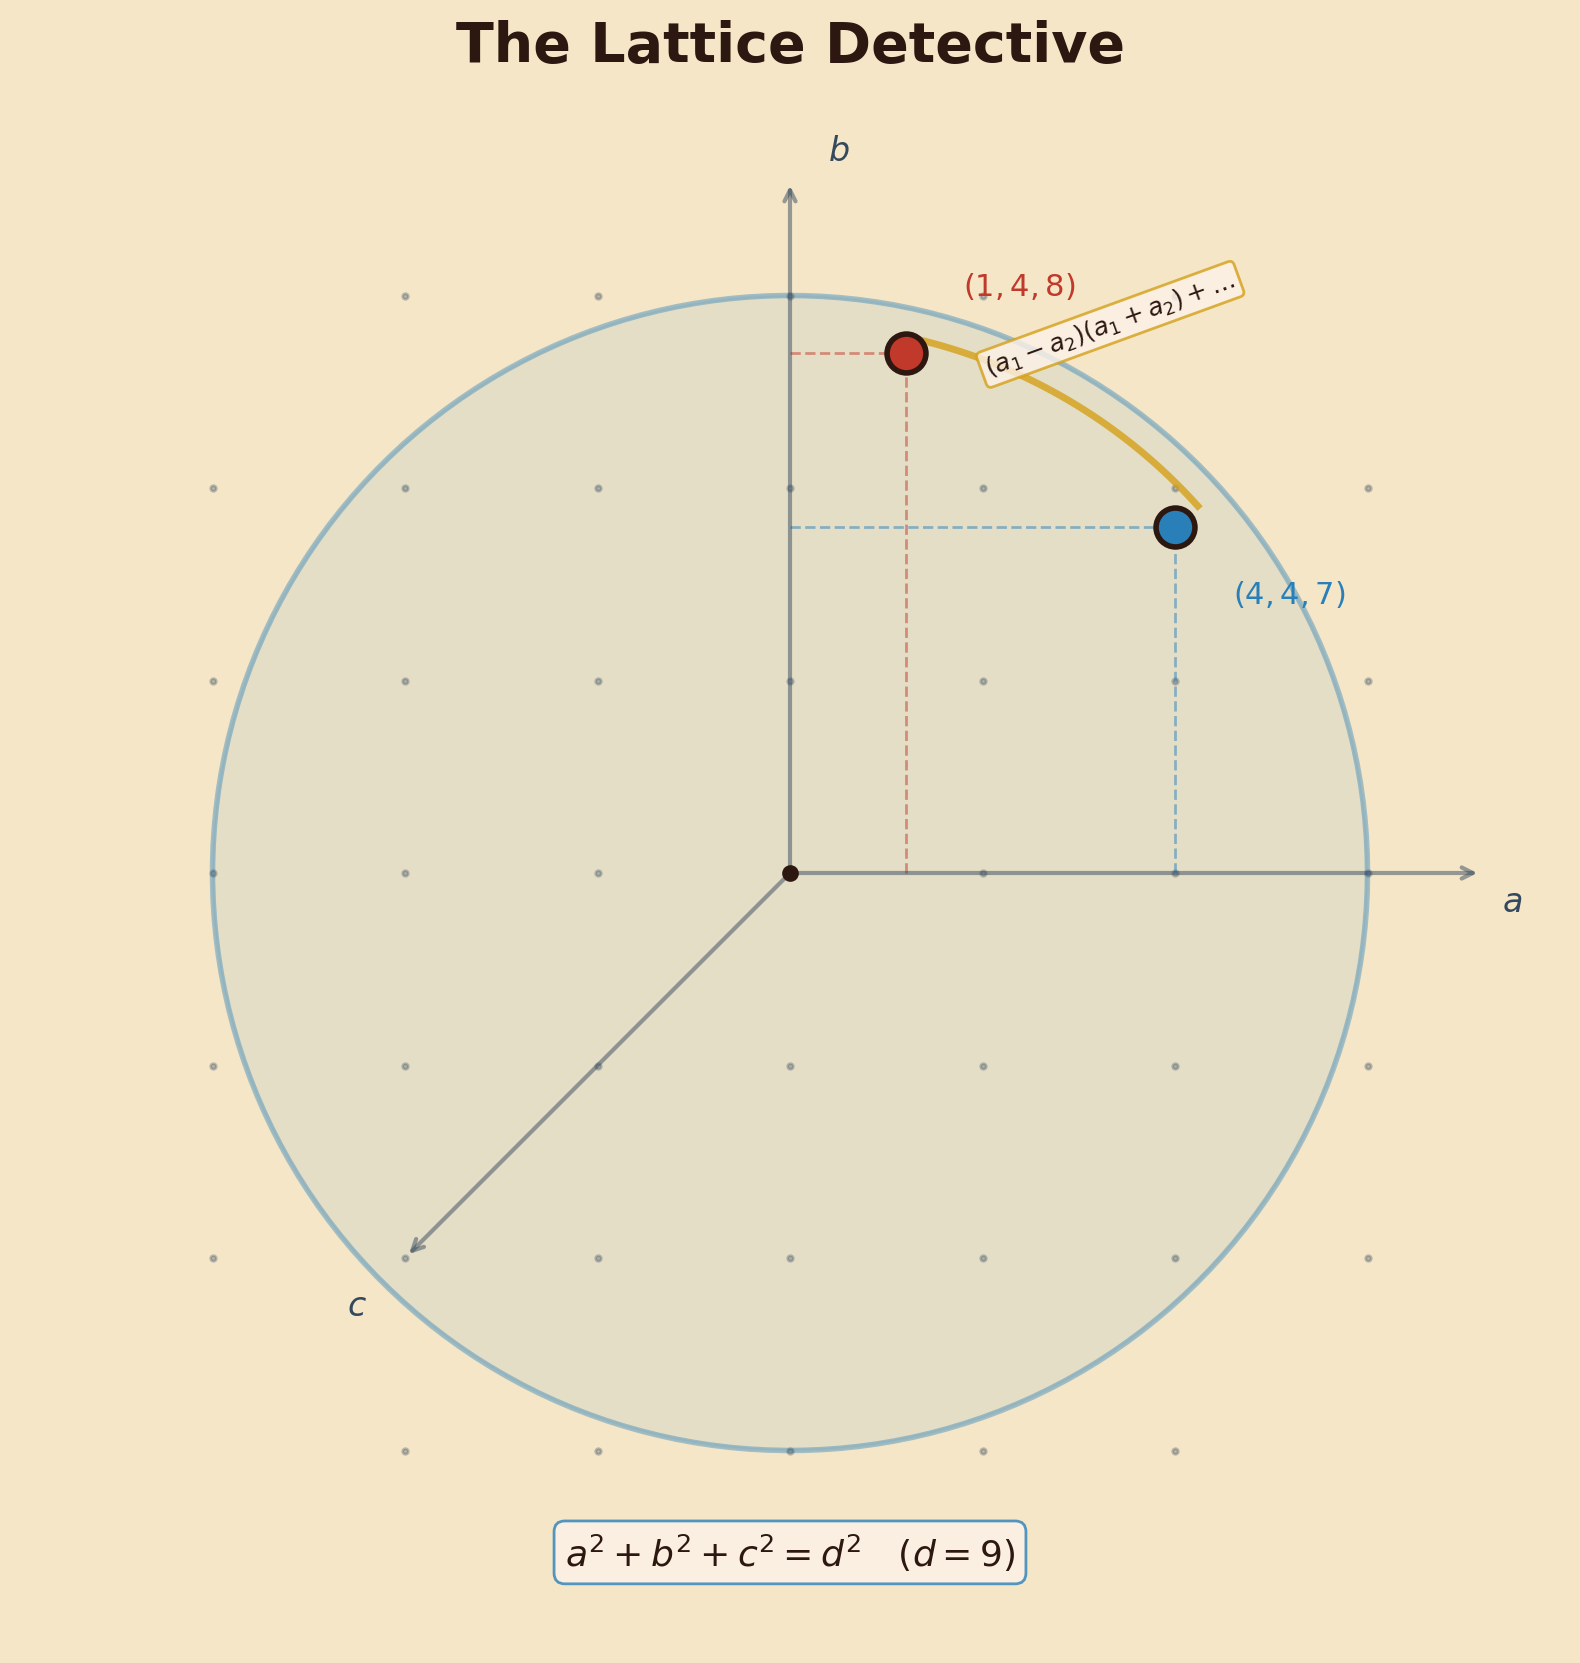
\includegraphics[width=0.82\textwidth]{../Chapter12/images/fig08_lattice_sphere.png}
\caption{A three-dimensional integer lattice (a grid of dots in space) with a translucent sphere of radius $d$ centred at the origin. Two lattice points on the sphere are highlighted in red and blue, with\ldots}
\end{figure}


\bigskip


\section{The Imaginary Witness}

In 1832, Carl Friedrich Gauss published a revolutionary paper on what he called \textit{complex integers} --- numbers of the form $a + bi$, where $a$ and $b$ are ordinary integers and $i = \sqrt{-1}$. Today we call them \textbf{Gaussian integers}, and they have their own private arithmetic: their own primes, their own notion of divisibility, their own version of unique factorisation. Gauss showed that the integer $5$, for instance, which is prime among the ordinary integers, \textit{splits} in the Gaussian world: $5 = (2 + i)(2 - i)$. The ordinary prime becomes a product of two Gaussian primes.
\index{Gaussian integers}

What does this have to do with Pythagorean quadruples? Everything. The \textbf{norm} of a Gaussian integer $z = a + bi$ is defined as

\[
N(z) = |z|^2 = a^2 + b^2.
\]

Now look at our bridge theorem: for any quadruple $(a, b, c, d)$,

\[
a^2 + b^2 = (d - c)(d + c).
\]

The left side is the Gaussian norm of $a + bi$. The right side is a factorisation in the ordinary integers. And $a + bi$ has its \textit{own} factorisation in the Gaussian integers: $a^2 + b^2 = (a + bi)(a - bi)$. So we arrive at the magnificent equation:

\[
(a + bi)(a - bi) = (d - c)(d + c).
\]

Two factorisations of the same number --- one in the Gaussian integers, one in the ordinary integers. Comparing them is precisely the trick Euler used to prove special cases of Fermat's theorems. The Gaussian integers are an \textit{imaginary witness}, testifying about the hidden structure of a number that the ordinary integers alone cannot reveal.
\index{Fermat, Pierre de}

Geometrically, the Gaussian integer $a + bi$ is a vector in the plane, and its norm $a^2 + b^2$ is the area of a square built on that vector. The factoring identity says: the area of that square equals the area of the rectangle with sides $(d - c)$ and $(d + c)$. Same area, different shape --- and the shape difference encodes the factors.

\begin{figure}[htbp]
\centering
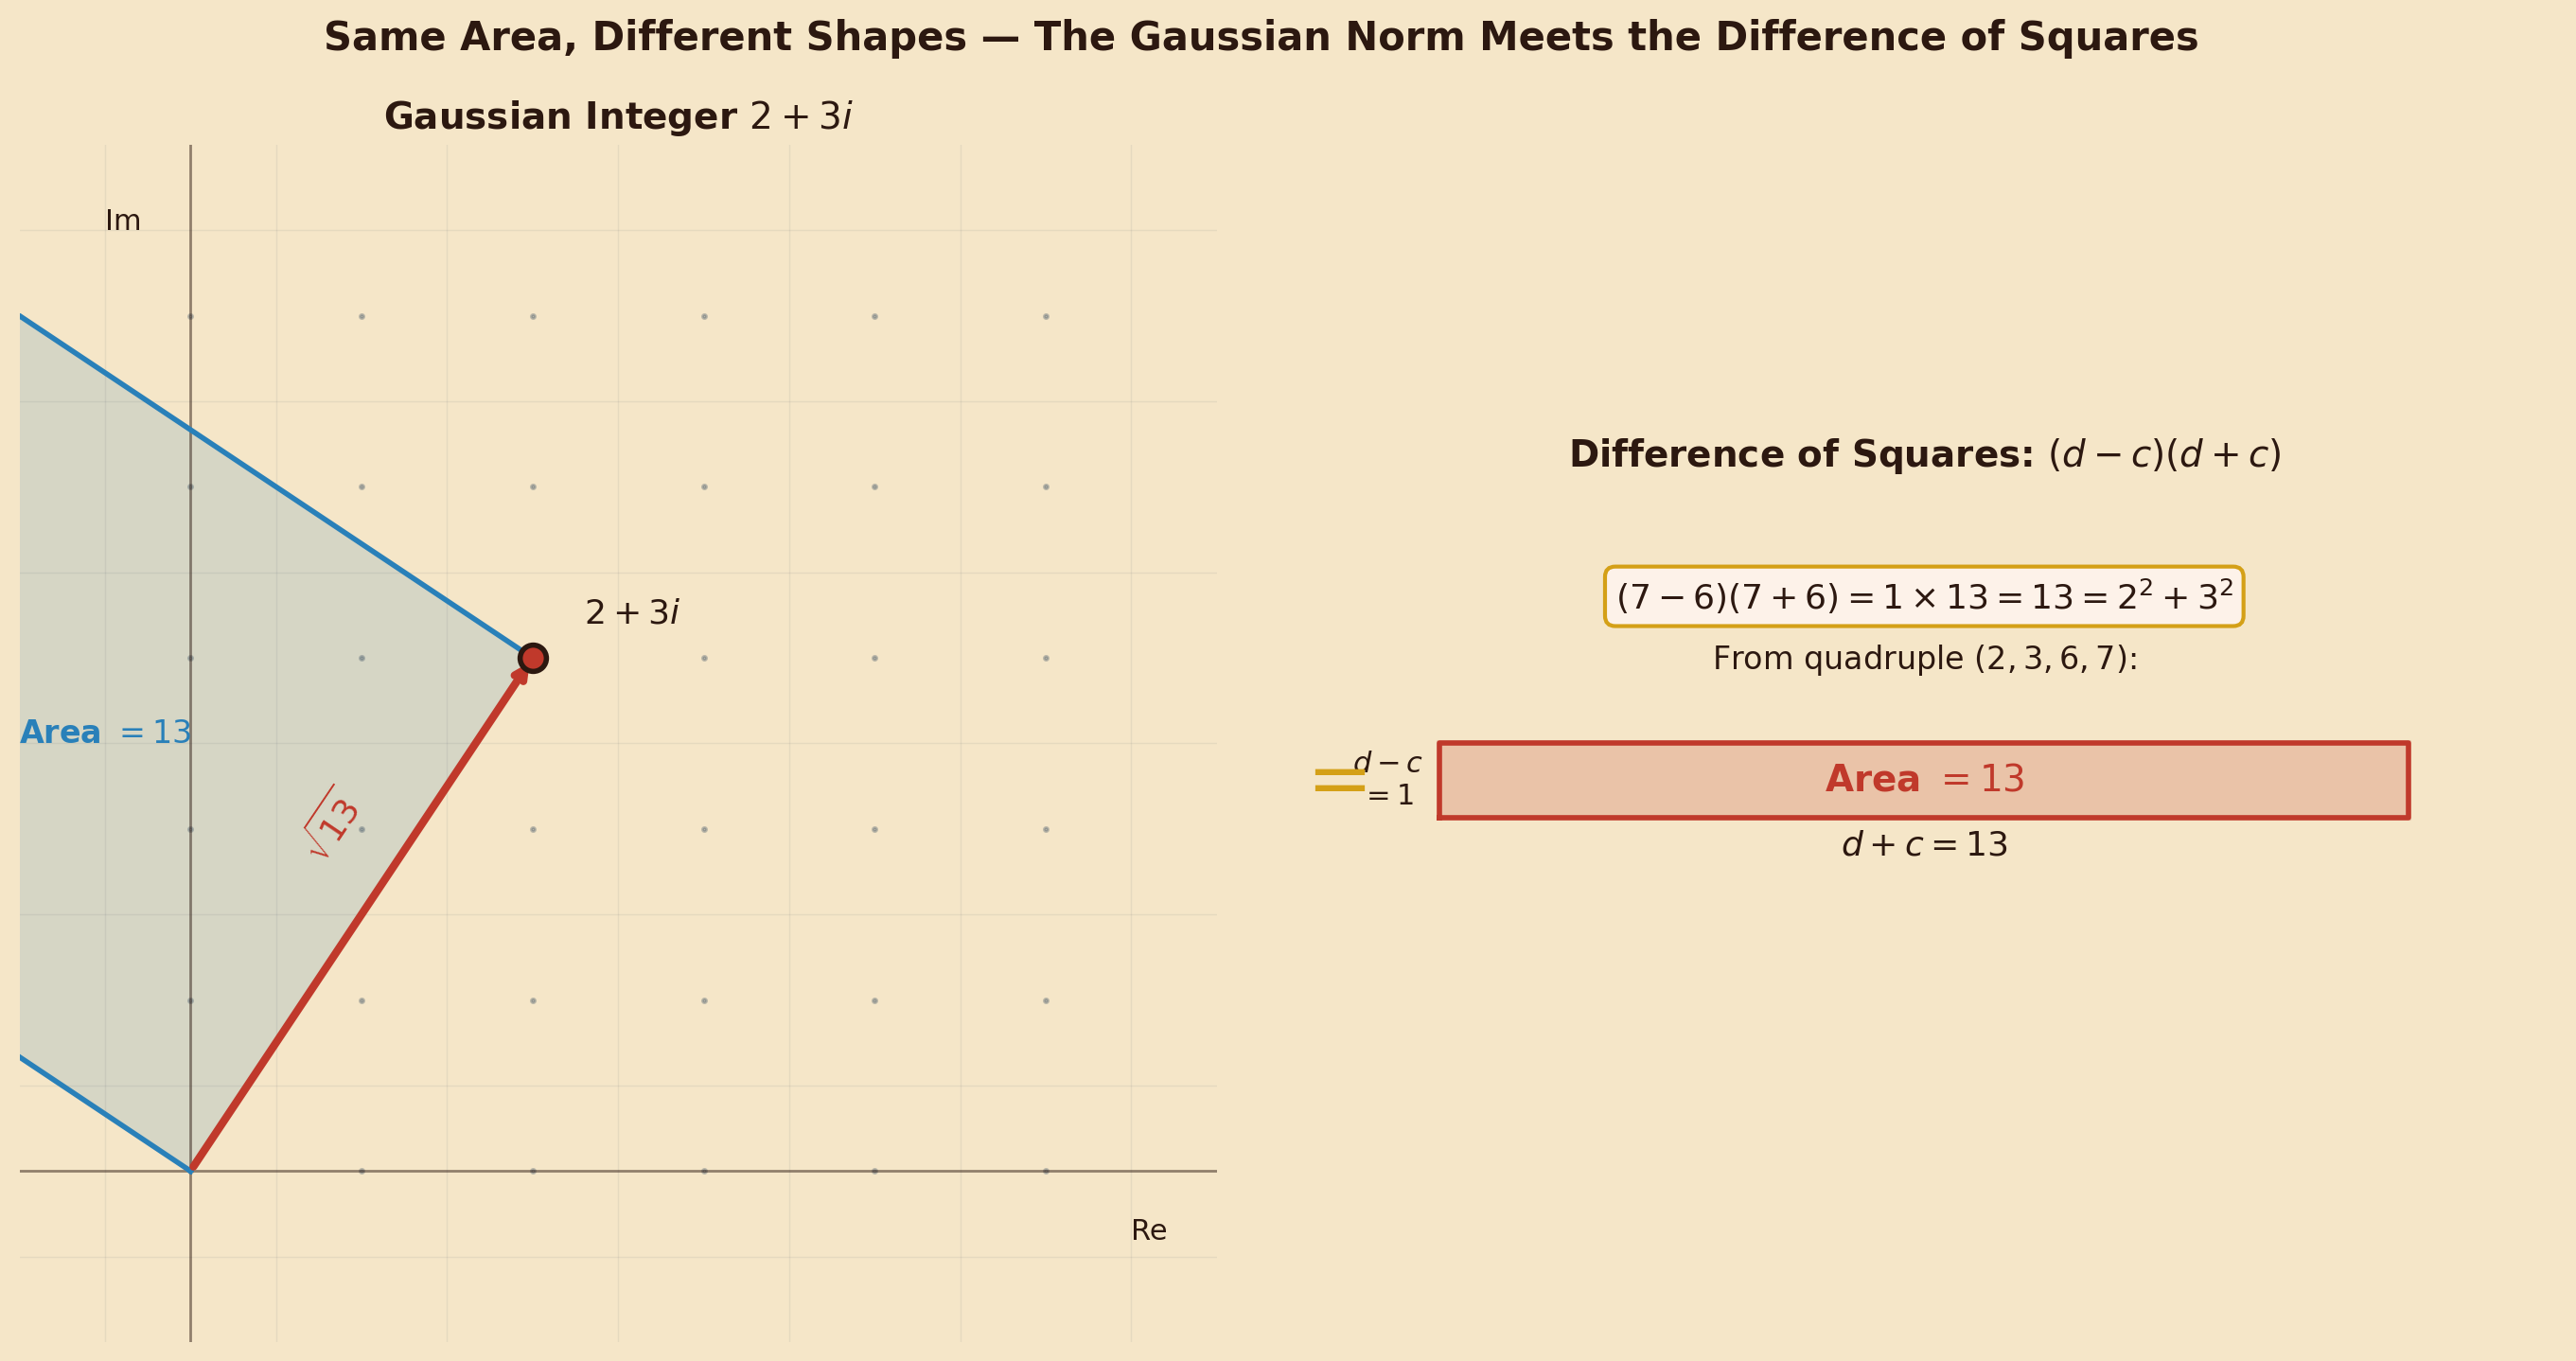
\includegraphics[width=0.82\textwidth]{../Chapter12/images/fig09_gaussian_plane.png}
\caption{The complex plane with an integer grid. A vector from the origin to the point $(2, 3)$ is drawn boldly, representing the Gaussian integer $2 + 3i$. A square of side length $\sqrt{13}$ is constructed\ldots}
\end{figure}


\bigskip


\section{The Prime Inquisitor}

"I'm thinking of two numbers," I say. "Their sum is $2d$ and their difference is $2c$." You look suspicious. "A prime $p$ divides their product. What can you deduce?"

Euclid knew the answer twenty-three centuries ago: if $p$ is prime and $p$ divides a product, then $p$ must divide at least one of the factors. This is \textbf{Euclid's Lemma} --- the oldest and sharpest lever in number theory. Applied to our Pythagorean bridge, it becomes a factoring crowbar.

From $(d - c)(d + c) = a^2 + b^2$, suppose a prime $p$ divides $a^2 + b^2$. Then $p$ divides the product $(d - c)(d + c)$, and Euclid's Lemma forces:

\[
p \mid (d - c) \qquad \text{or} \qquad p \mid (d + c).
\]

This is the \textbf{Prime Divisor Dichotomy} --- every prime factor of $a^2 + b^2$ must "choose a side," landing in either the gap $(d - c)$ or the sum $(d + c)$. And once it chooses, we can extract it by GCD.

Two small lemmas sharpen the blade. If $p$ divides \textit{both} $(d - c)$ and $(d + c)$, then:

\begin{itemize}
\item $p$ divides their sum: $(d - c) + (d + c) = 2d$.
\item $p$ divides their difference: $(d + c) - (d - c) = 2c$.
\end{itemize}
So a prime that divides both factors must divide $2d$ and $2c$. If $p$ is odd, this means $p \mid d$ and $p \mid c$ --- the prime is a common factor of the hypotenuse and the third leg. For \textit{primitive} quadruples (where $\gcd(a, b, c, d) = 1$), such sharing is severely constrained.

A worked example: the quadruple $(2, 3, 6, 7)$ gives $a^2 + b^2 = 13$, which is prime. So $13 \mid (7 - 6) = 1$ or $13 \mid (7 + 6) = 13$. The latter holds. Now $\gcd(13, 7) = 1$, confirming that $7$ is coprime to $13$ --- consistent with $7$ being prime.

For a \textit{composite} hypotenuse, the lever pries harder. If $d = 15$ and we find a quadruple with $a^2 + b^2$ divisible by $3$ or $5$, the GCD computation $\gcd(d - c, d)$ or $\gcd(d + c, d)$ will yield a non-trivial factor. The prime inquisitor always extracts a confession.

\begin{figure}[htbp]
\centering
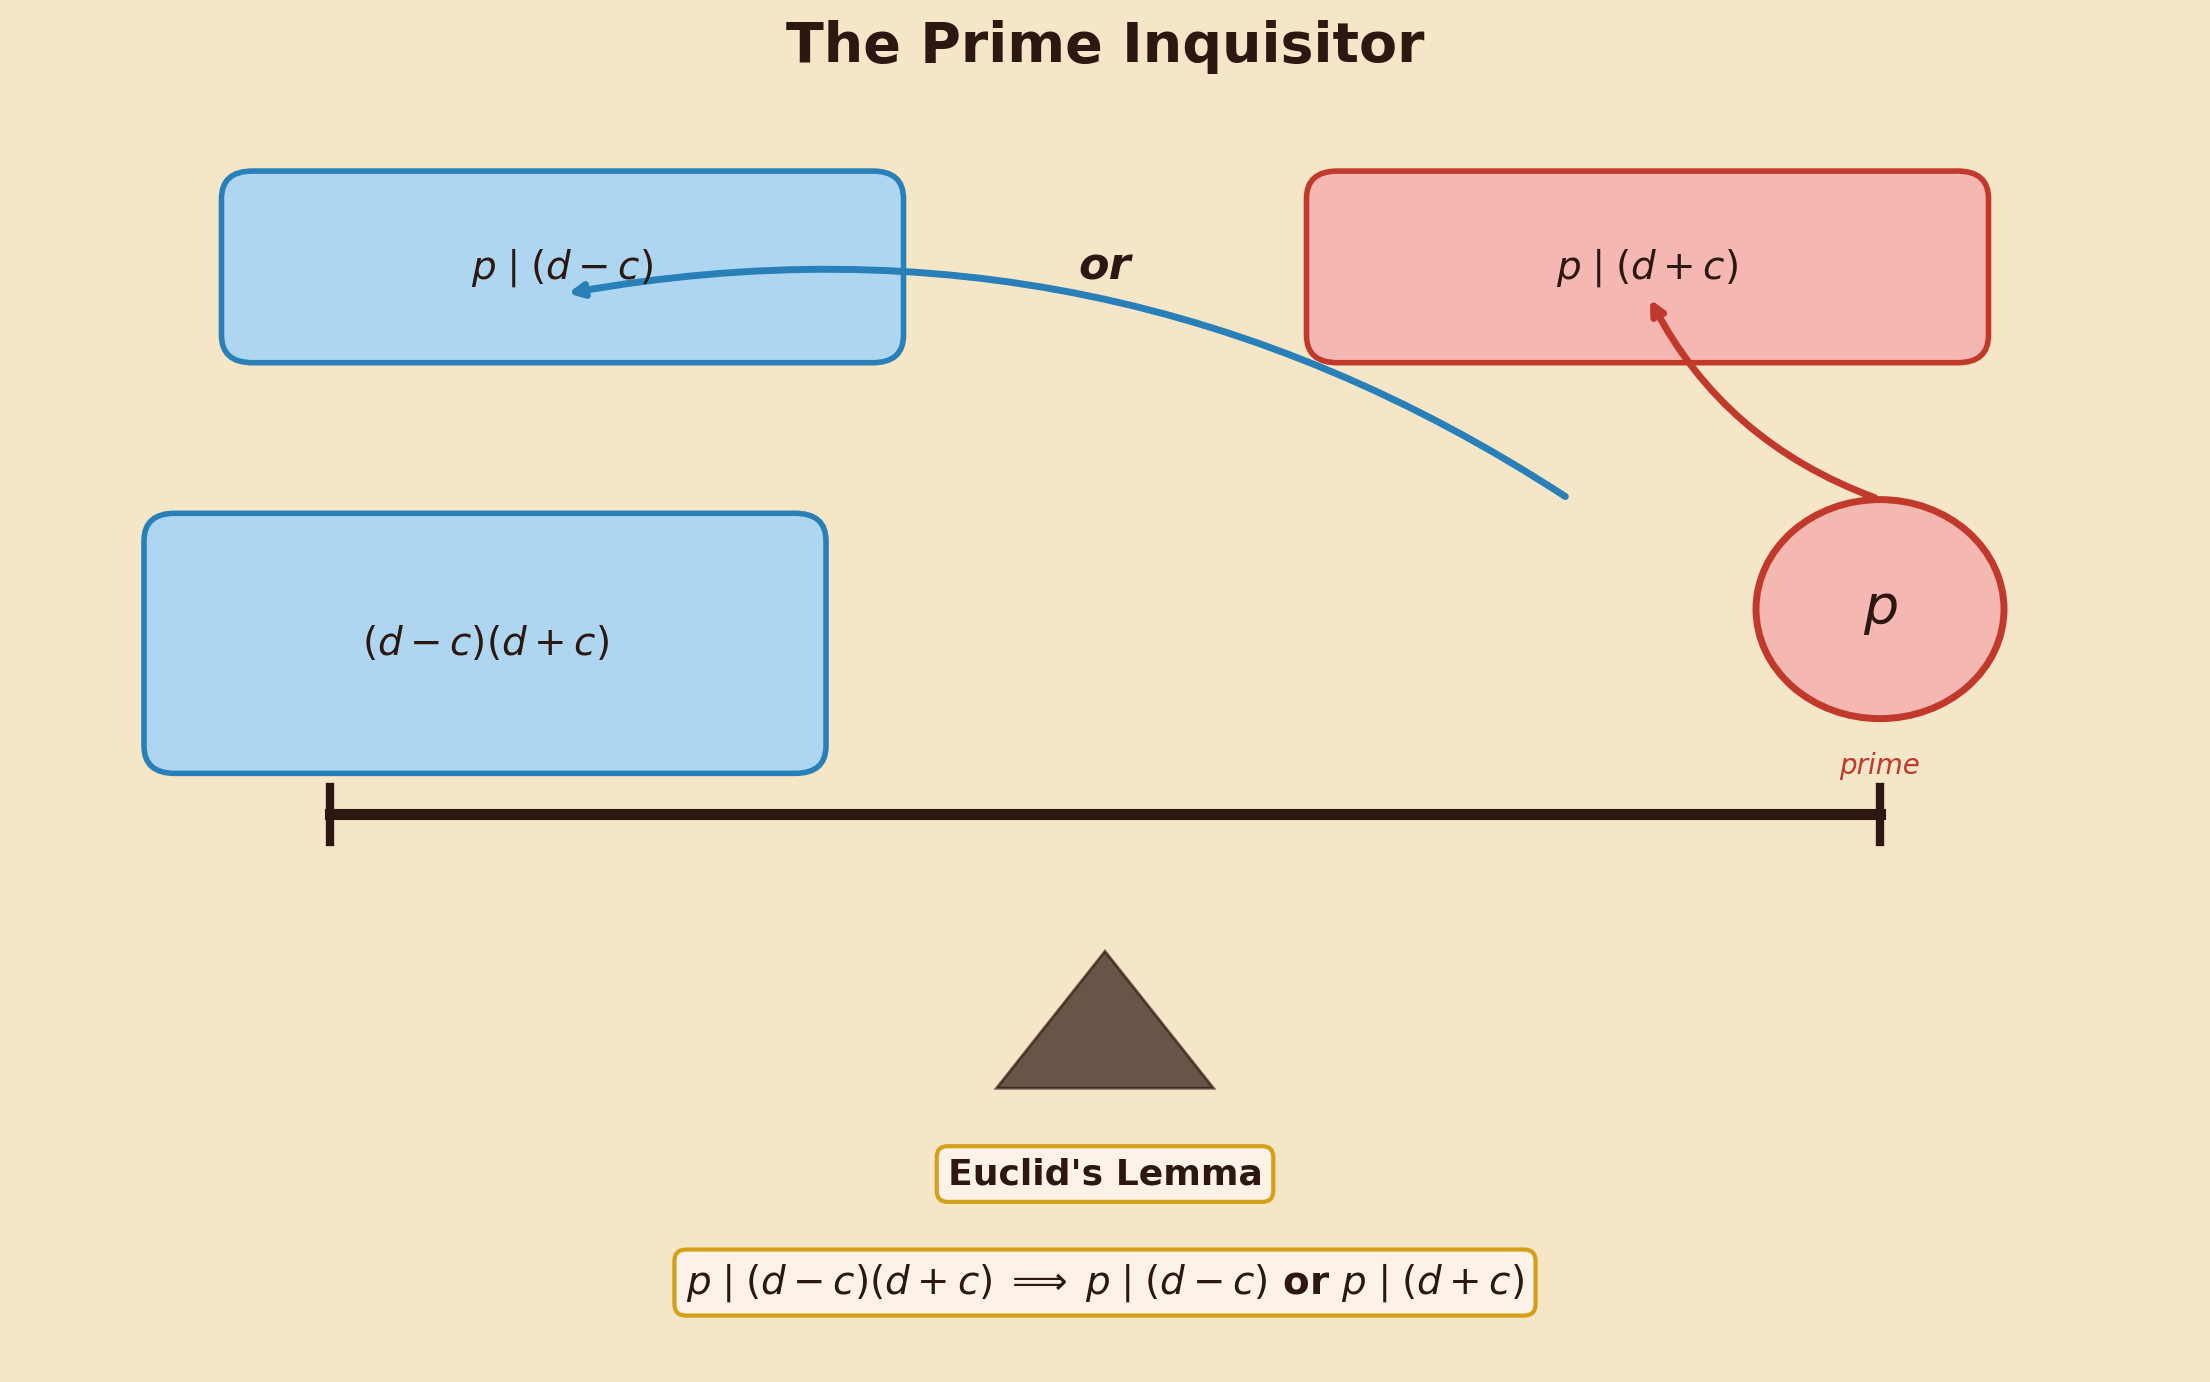
\includegraphics[width=0.82\textwidth]{../Chapter12/images/fig10_euclid_lever.png}
\caption{An Archimedes-style lever diagram. A beam balances on a triangular fulcrum labelled "Euclid's Lemma." On the left end of the beam sits the product $(d - c)(d + c)$; on the right, a weight labelled\ldots}
\end{figure}


\bigskip


\section{The Mod Squad}

Quick: can $7^2 + 7^2 + 7^2$ be a perfect square? Compute: $49 + 49 + 49 = 147$. Is $147$ a perfect square? No --- $12^2 = 144$ is too small and $13^2 = 169$ is too large. But is there a deeper reason, an \textit{obstruction} that rules out such quadruples before we ever touch a calculator?

There is, and it lives in the arithmetic of remainders. Every perfect square, when divided by $4$, leaves a remainder of $0$ or $1$. (Check: $0^2 = 0$, $1^2 = 1$, $2^2 = 4 \equiv 0$, $3^2 = 9 \equiv 1$, and the pattern repeats.) So the sum $a^2 + b^2 + c^2$, modulo $4$, can be $0$, $1$, $2$, or $3$ --- but $d^2$ can only be $0$ or $1$. Therefore:

\[
a^2 + b^2 + c^2 \equiv 0 \;\text{or}\; 1 \pmod{4}
\]

is a \textit{necessary} condition for any Pythagorean quadruple. Now, $7^2 + 7^2 + 7^2 \equiv 1 + 1 + 1 = 3 \pmod{4}$. The mod $4$ obstruction kills it instantly --- no calculator required.

When all four components are even, something elegant happens. Write $a = 2a'$, $b = 2b'$, $c = 2c'$, $d = 2d'$. Then $4a'^2 + 4b'^2 + 4c'^2 = 4d'^2$, and dividing through by $4$ gives $a'^2 + b'^2 + c'^2 = d'^2$. The quadruple \textit{descends} to a smaller one. This "mod $2$ descent" can be repeated until at least one component is odd --- reaching the primitive core.

Legendre proved a famous and beautiful theorem: an integer $n$ is a sum of three squares if and only if $n$ is \textit{not} of the form $4^k(8m + 7)$ for non-negative integers $k$ and $m$. This classical result constrains which $d^2$ can be written as $a^2 + b^2 + c^2$, and therefore which composite numbers $d$ are amenable to the quadruple factoring method. The modular world is the gatekeeper, deciding who may enter the world of quadruples --- and who must be turned away.

\begin{figure}[htbp]
\centering
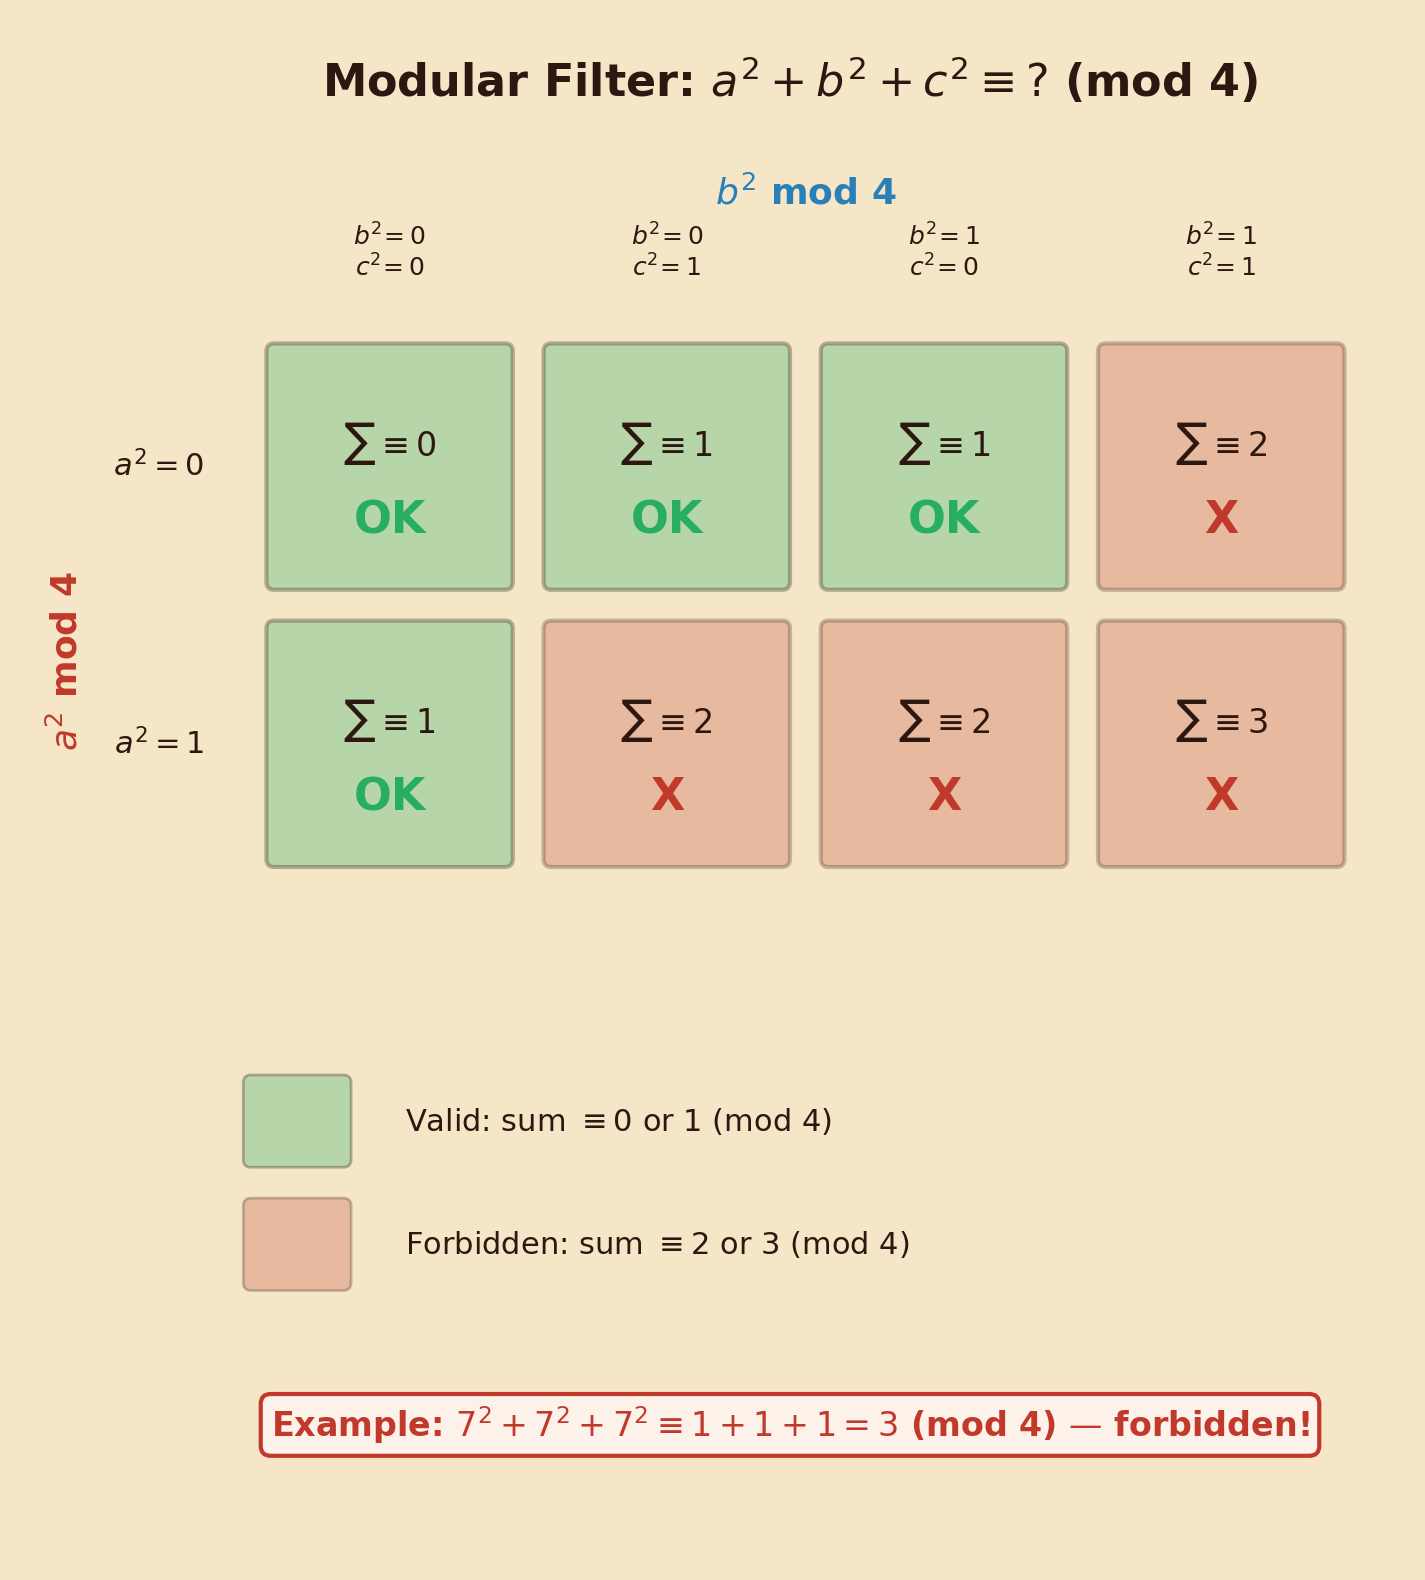
\includegraphics[width=0.82\textwidth]{../Chapter12/images/fig11_mod4_grid.png}
\caption{A $4 \times 4$ grid where rows represent values of $a^2 \bmod 4$ (labelled $0$ and $1$, repeating) and columns represent $b^2 \bmod 4$. Each cell contains two sub-cells for the two possible values of\ldots}
\end{figure}


\bigskip


\section{The Number Cruncher's Workbench}

The mathematician's motto: \textit{trust, but verify}. Let us now roll up our sleeves, sharpen our pencils, and put every theorem in this chapter through the wringer.

\textbf{Difference-of-squares check.} For each of our four showcase quadruples:
\index{difference of squares}

\[
\begin{aligned}
(1,2,2,3): &\quad (3-2)(3+2) = 1 \times 5 = 5 = 1 + 4. \quad \checkmark \\
(2,3,6,7): &\quad (7-6)(7+6) = 1 \times 13 = 13 = 4 + 9. \quad \checkmark \\
(1,4,8,9): &\quad (9-8)(9+8) = 1 \times 17 = 17 = 1 + 16. \quad \checkmark \\
(4,4,7,9): &\quad (9-7)(9+7) = 2 \times 16 = 32 = 16 + 16. \quad \checkmark
\end{aligned}
\]

**Collision check for $d = 9$.** From quadruples $(1,4,8,9)$ and $(4,4,7,9)$:

\[
(8-7)(8+7) = 15, \qquad (4^2 - 1^2) + (4^2 - 4^2) = 15. \quad \checkmark
\]

And $\gcd(15, 81) = 3$. Factor extracted.

\textbf{Lattice identity.} $(1-4)(1+4) + (4-4)(4+4) = -15 = (7-8)(7+8)$. $\checkmark$

\textbf{Gaussian norm.} $2 + 3i$ has norm $4 + 9 = 13 = (7-6)(7+6)$. $\checkmark$


\bigskip


The chapter closes with a set of challenges for the ambitious reader:

\begin{enumerate}
\item Find a Pythagorean quadruple with $d = 15$ and use it to find a non-trivial factor of $15$.
\item Find \textit{two} quadruples with $d = 21$ and apply the collision theorem.
\item Verify the parametric formula for $m = 2$, $n = 1$, $p = 1$, $q = 1$.
\item Prove that no Pythagorean quadruple with $a = b = c$ can have $d$ prime. *(Hint: consider the equation modulo $3$.)*
\item Find the smallest $d$ with three or more distinct primitive quadruples.
\item Use the Gaussian-integer bridge to show that $5 = (2 + i)(2 - i)$ and connect this to a quadruple with $a^2 + b^2 = 5$.
\item Determine all $d \le 20$ for which Pythagorean quadruples exist.
\item \textit{(Open)} Is there an efficient algorithm to enumerate all primitive Pythagorean quadruples with hypotenuse $d$ in time polynomial in $\log d$?
\end{enumerate}
\begin{figure}[htbp]
\centering
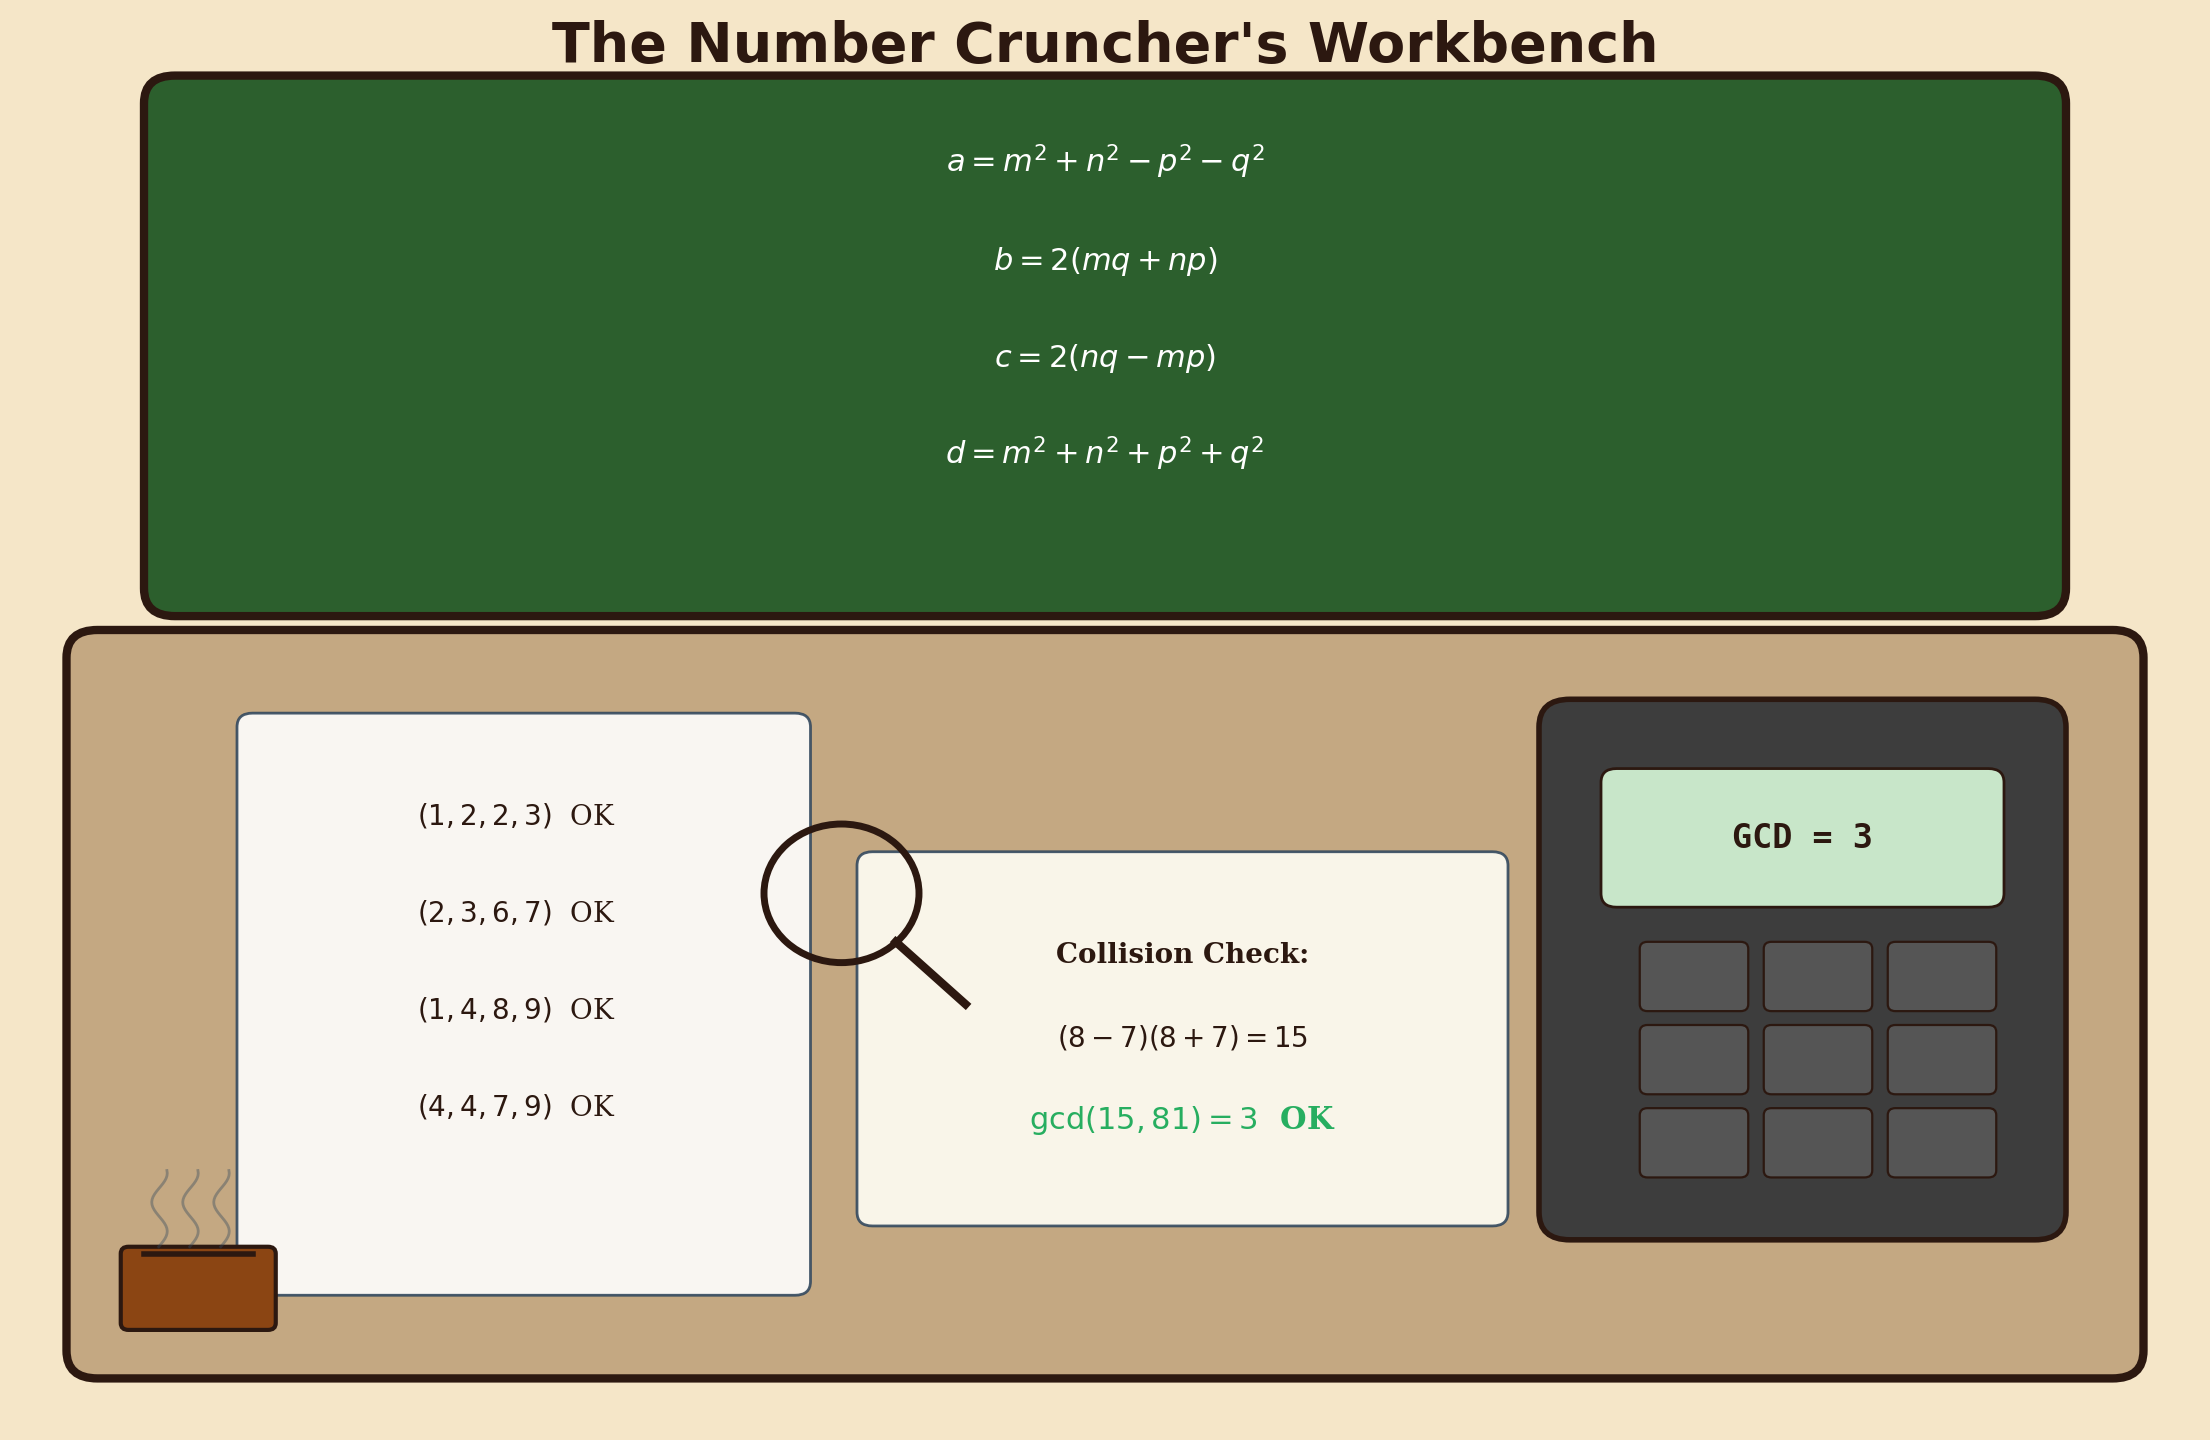
\includegraphics[width=0.82\textwidth]{../Chapter12/images/fig12_workbench.png}
\caption{A mathematician's workbench scene. A wooden desk is strewn with papers showing the four showcase quadruples, pencil stubs, and a magnifying glass poised over the collision identity. A chalkboard in\ldots}
\end{figure}

\begin{figure}[htbp]
\centering
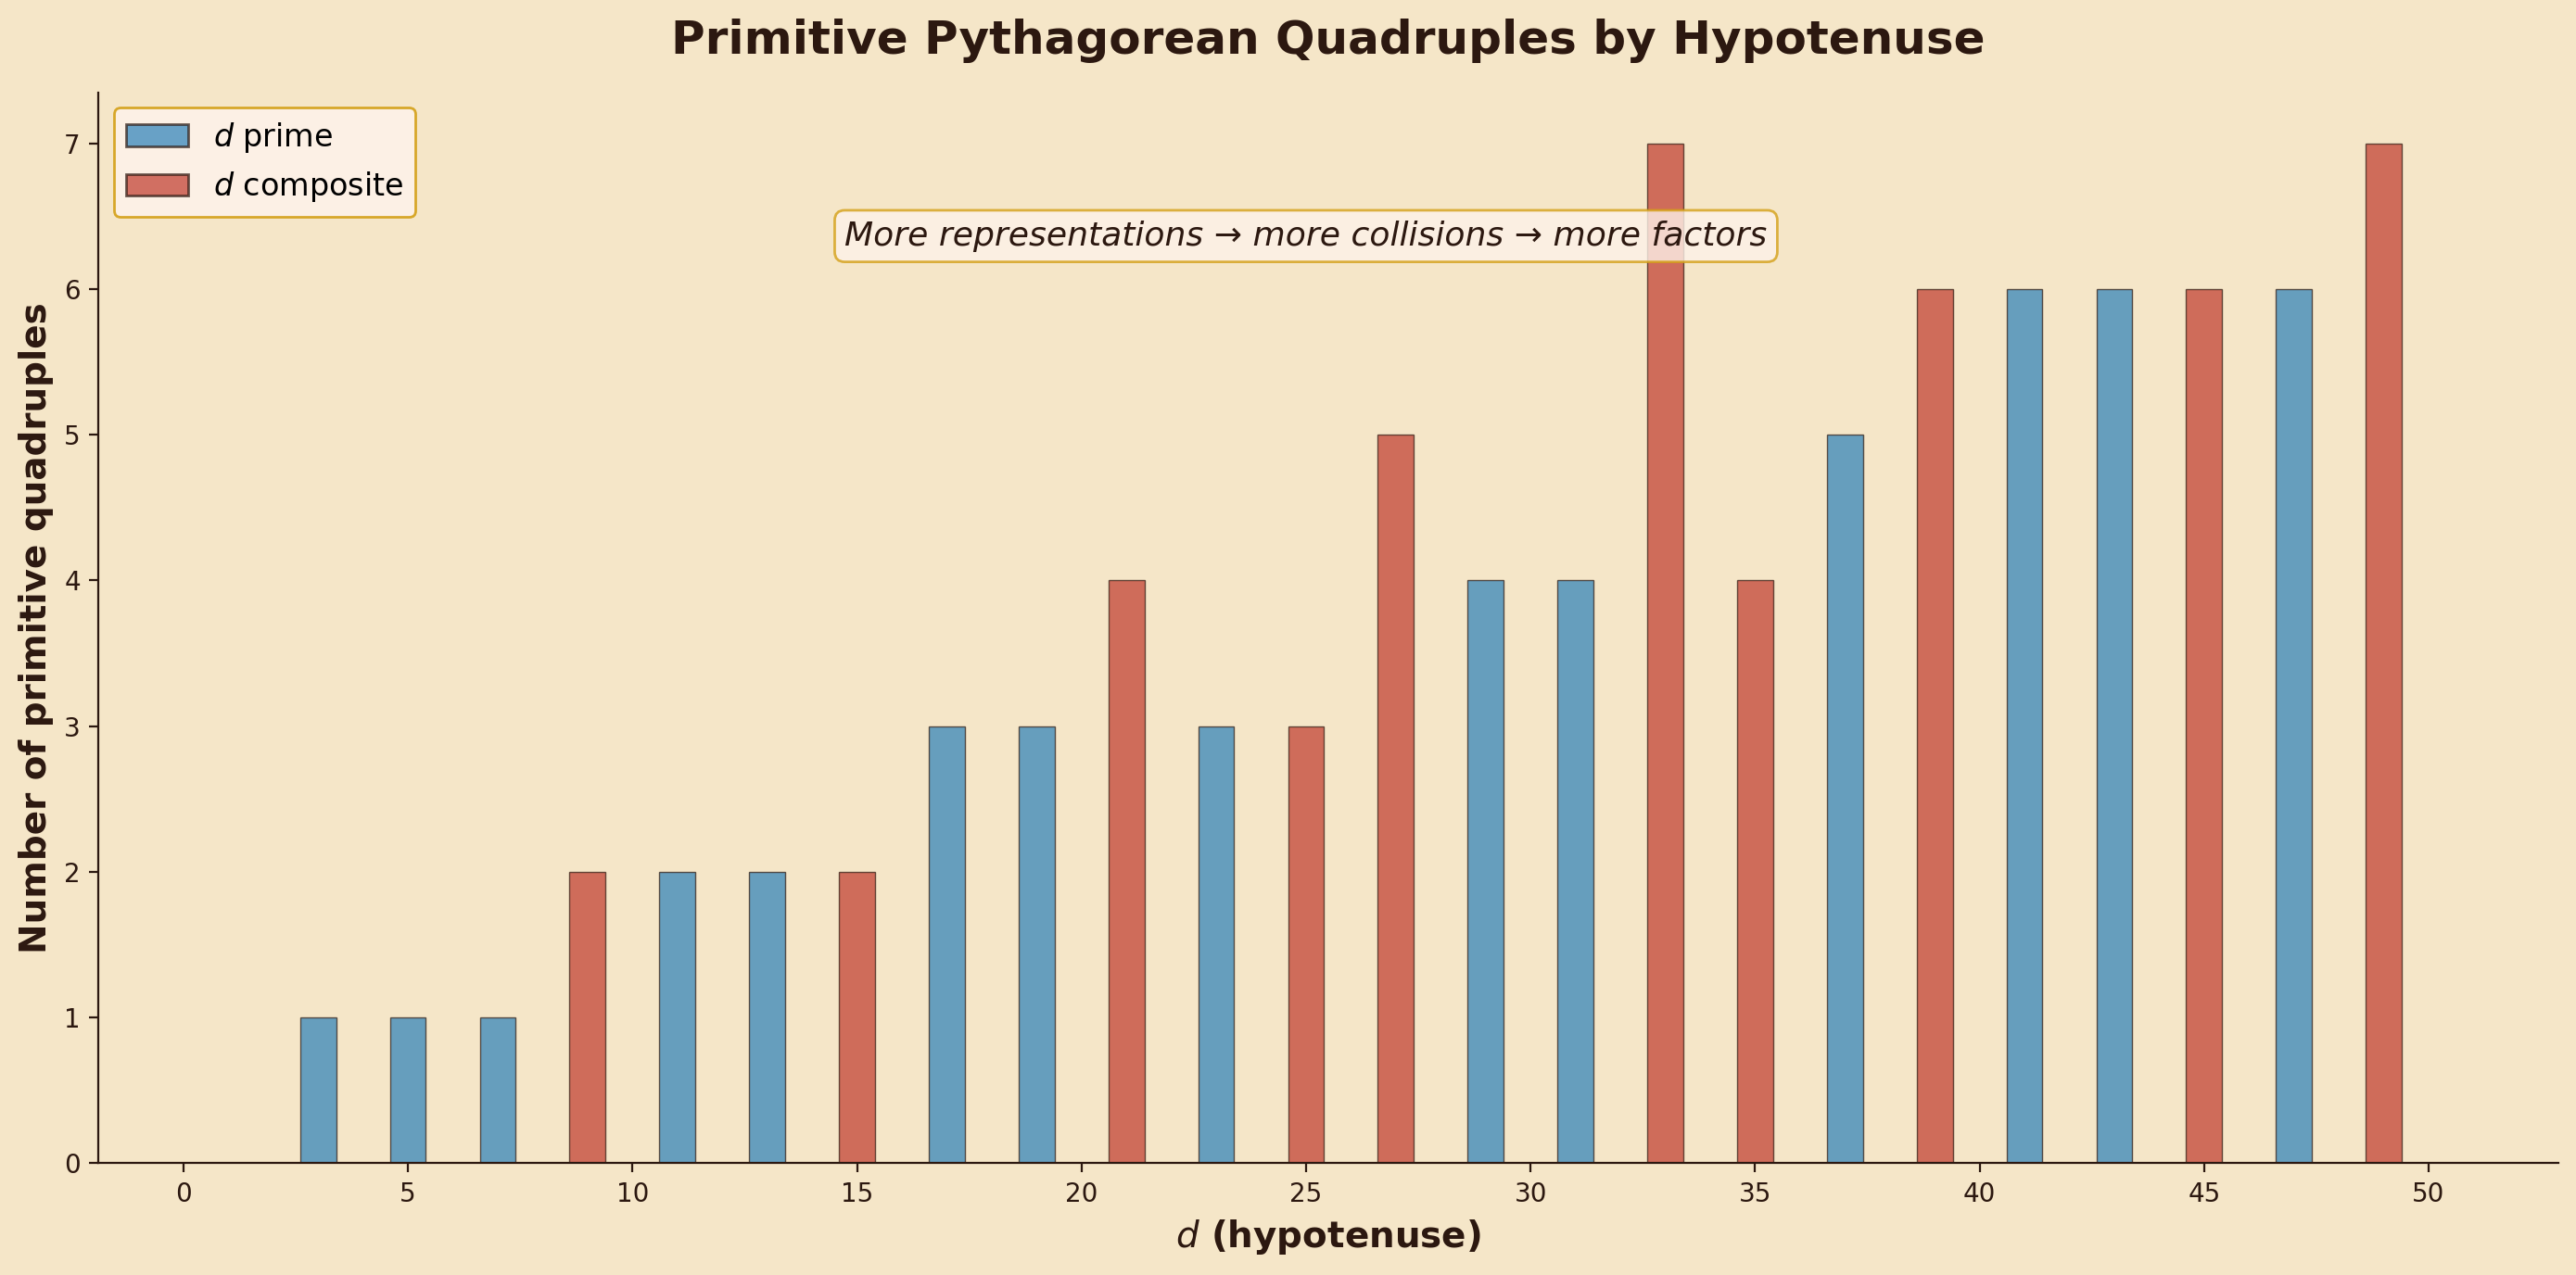
\includegraphics[width=0.82\textwidth]{../Chapter12/images/fig13_histogram.png}
\caption{A histogram (bar chart) showing the number of primitive Pythagorean quadruples for each value of $d$ from $1$ to $50$. Bars for prime values of $d$ are coloured blue; bars for composite values of $d$\ldots}
\end{figure}


\bigskip


These ten theorems --- the bridge, the machine, the collision, the scaling law, the lattice identity, the Gaussian witness, the prime inquisitor, the modular filter, and their verifications --- are not museum pieces. They are the moving parts of a \textit{factoring engine}. In the next chapter, we will assemble them into a working mechanism: the \textbf{GCD Cascade}, a systematic procedure for extracting the prime factors of a composite number from the web of relationships hidden inside its Pythagorean quadruples. The journey from four wooden blocks on a table to the breaking of composite numbers is shorter than you might think --- and far more beautiful.
\index{GCD cascade}

